\chapter{Experiments and Results}
\label{chapter:chapter05}

This chapter represents the core experiments of the research. The main purpose of it was to do a benchmark, as a starting point for the comparison between SOAs and MOAs. The basis for the experimentation layout was based on the experimental framework proposed by H. Ishibuchi, Y. Nojima and T. Doi~\cite{Ishibuchi_single_vs_multiobjective}. \\

The chapter is divided into four different sections, described below:

\begin{itemize}
    \item \textbf{Experiments setup} consists of a set of experiments to determine a reference front to use it for comparison against SOAs and MOAs.
    \item \textbf{First phase} consists of the run of the algorithms without any adjustment using the parameters found in the experimental setup for all the algorithms. This also includes an analysis of the stability of some of the resulting groups.
    \item \textbf{Second phase} takes into account the results of the first phase of experiments and feedback made for its results. It discusses one of the main issues made by the feedback which remarks on whether or not the comparison between SOA and MOA was fair.
    \item \textbf{Third phase} is the result of a discussion about the tuning of parameters. Using only the best algorithms from phase one, chosen by their performance using the parameters from the Experimental setup. 
\end{itemize}

\section{Experiments Setup}

The next section discusses a set of experiments that took place before the core experiments could be made. The first subsection shows the experiment made to search for a reference front for the performance comparison. The next subsection shows an experiment for obtaining the base parameters that would be used to have a fair comparison between the algorithms. The last subsection discusses some of the specific details about each of the individual algorithm implementations.

\subsection{Searching for a Reference Pareto Front}

The IGD+ metric requires to have a defined reference front to perform a proper comparison. To this end, the NSGA-II algorithm was used with a population of 20 individuals for 1000 generations, across 200 independent runs. The best front was chosen considering their HV for each of the problem sizes.\\

After the experiment, the results of each run were compared with each other, and the ones with the lowest HV were chosen. These results are shown in Figures~\ref{fig:reference_front_20}~to~\ref{fig:reference_front_2000} for each respective problem. An important observation is that, in n=20 and n=200, some of the individuals had the same value for each of their objective functions. This observation is important because it is an indication that a global minimum for these problems may exist and could be found using an SOA.\\

\begin{figure}[H]
    \centering
    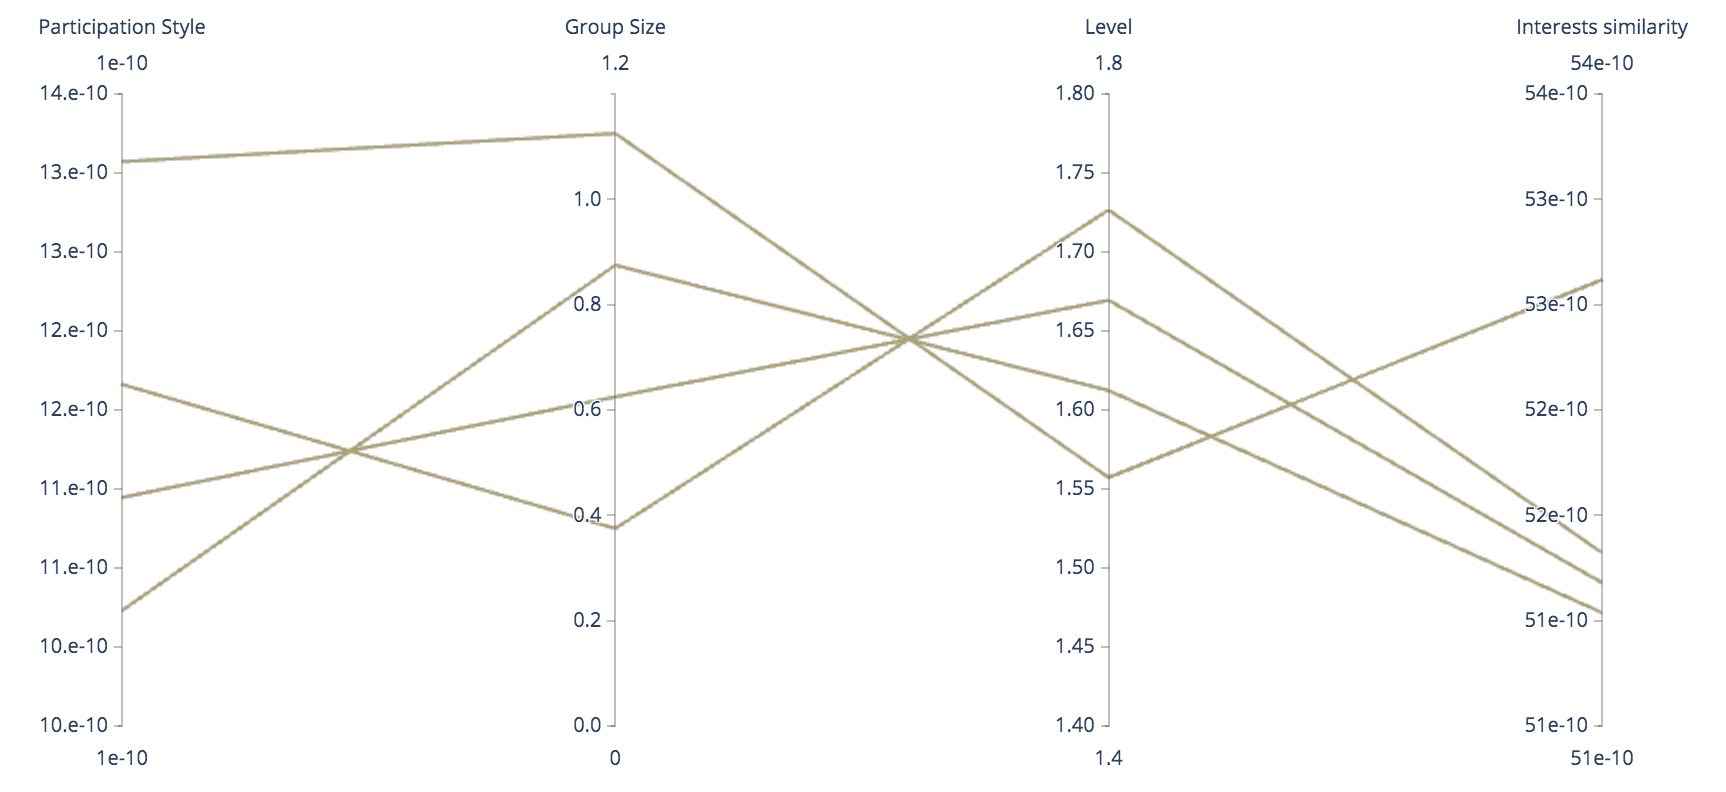
\includegraphics[width=\textwidth]{images/parallel_ref_20.png}
    \caption{Reference front for the $n=20$ problem.}
    \label{fig:reference_front_20}
\end{figure}

\begin{figure}[H]
    \centering
    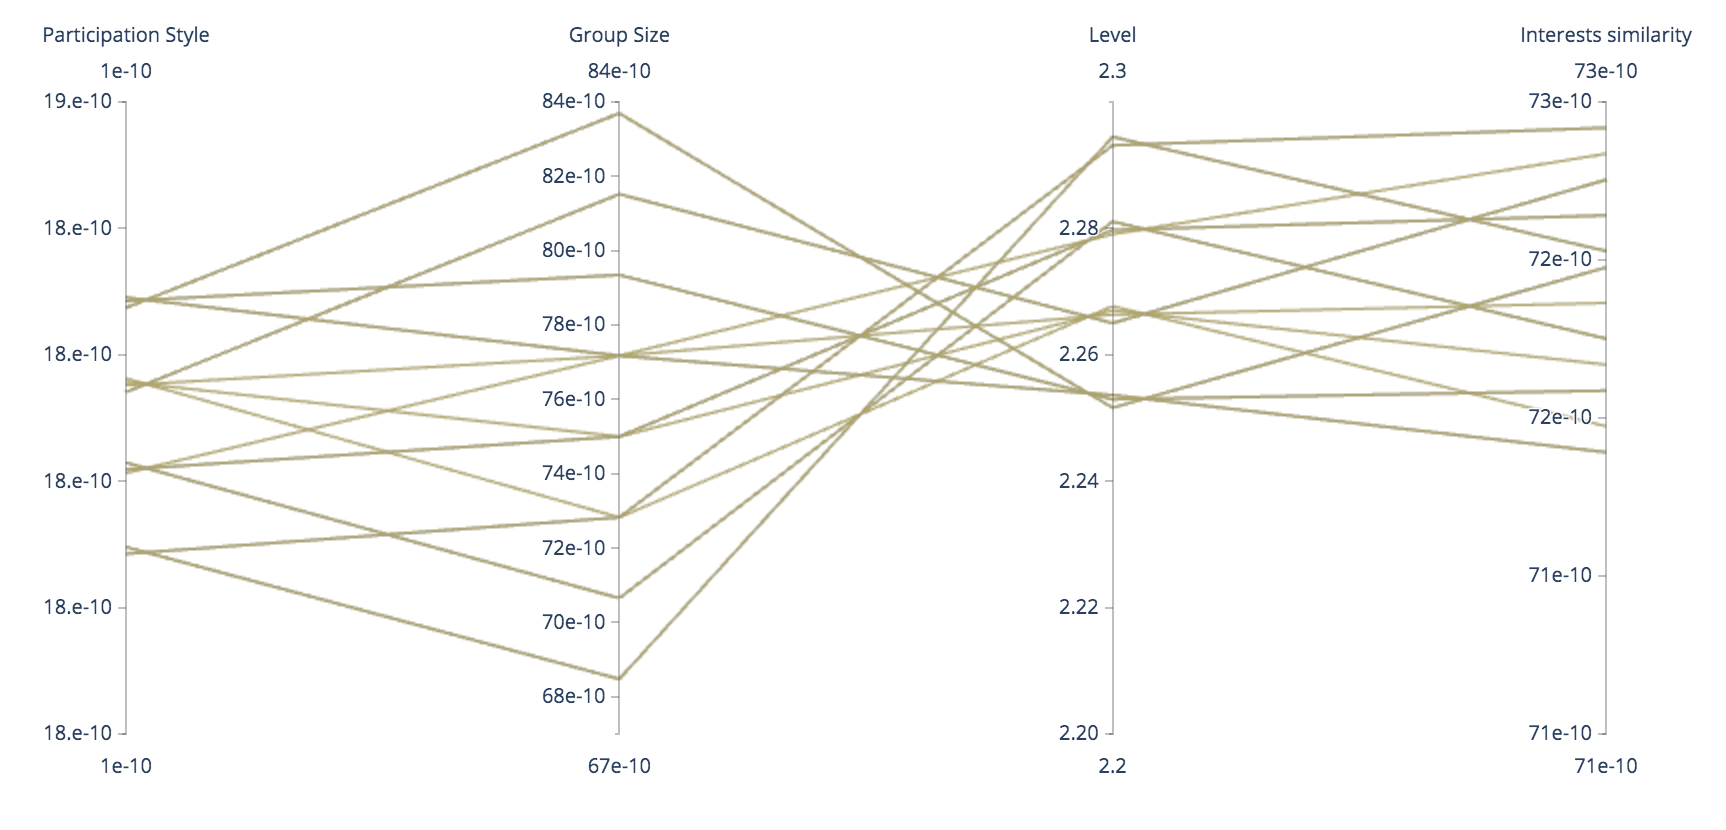
\includegraphics[width=\textwidth]{images/parallel_ref_200.png}
    \caption{Reference front for the $n=200$ problem. }
    \label{fig:reference_front_200}
\end{figure}

\begin{figure}[H]
    \centering
    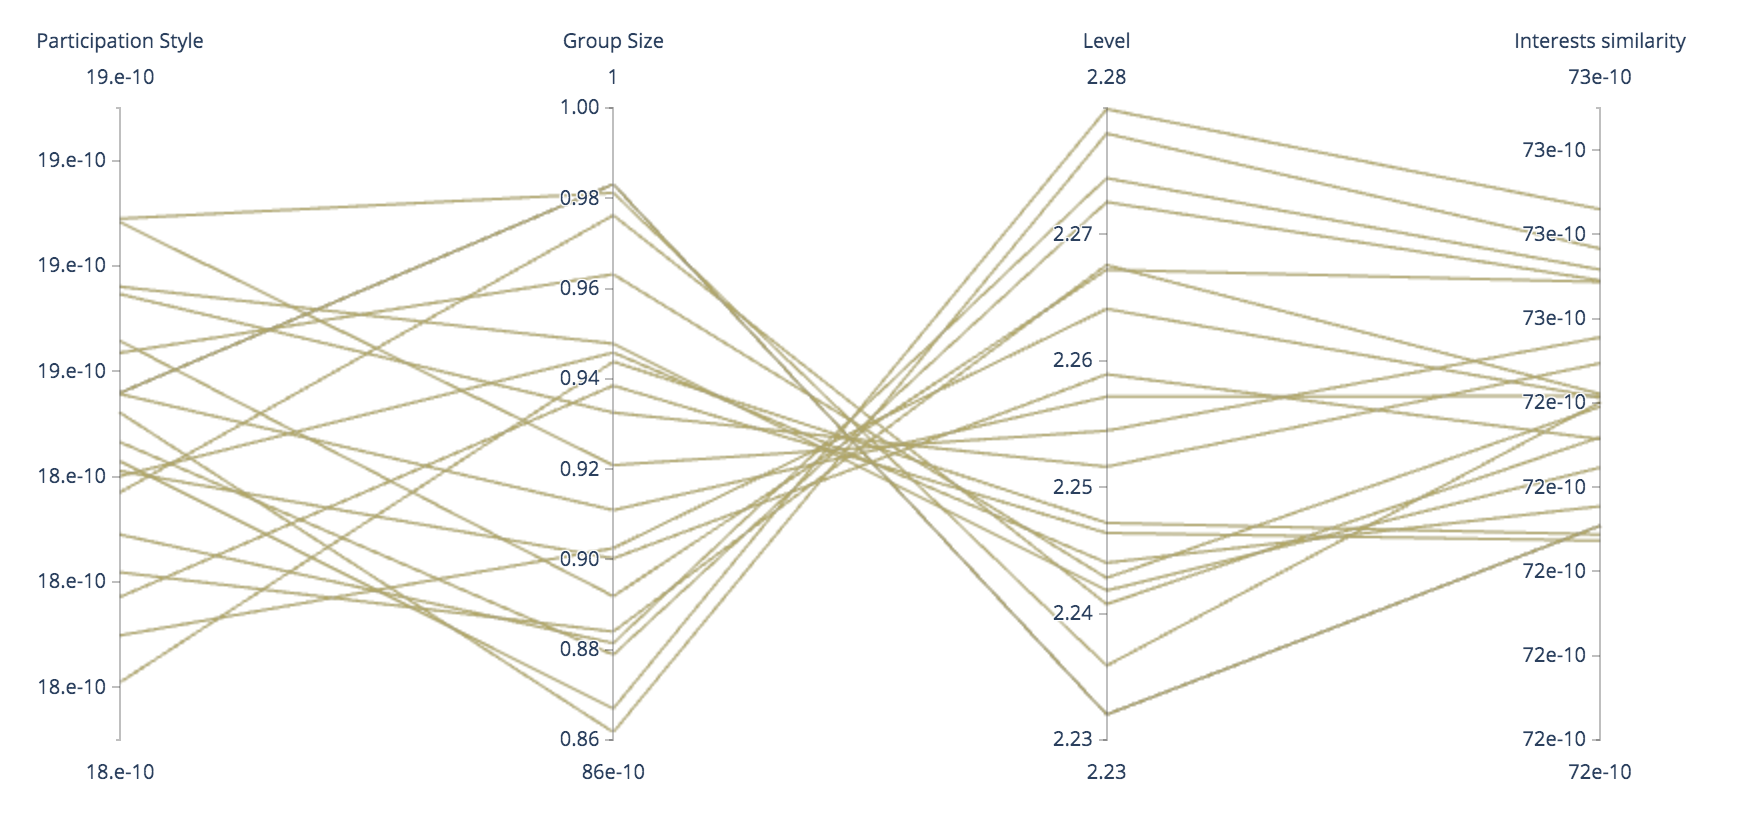
\includegraphics[width=\textwidth]{images/parallel_ref_2000.png}
    \caption{Reference front for the $n=2,000$ problem. }
    \label{fig:reference_front_2000}
\end{figure}

\subsection{Searching for Reference Parameters}

After some empiric testing with several values for the number of generations or steps $s$ and the population size $p$, there was a significant rise in complexity, especially for the high problem of $n=2,000$. This resulted in some experiments running for several hours and an overuse of memory space, even after using memorisation for the evaluation of costly objective functions. So, there is a bias to chose a pair small enough to maintain the complexity low, but high enough to produce a significant comparison.\\

Considering that a fair comparison requires a level of complexity similar to each algorithm, this research used the same parameters for $s$ and $p$, and the same operators for each of the algorithms. It should be noted that not all the algorithms used both of these parameters, but they were considered because they were shared across most of the algorithms.\\

In this experiment, several combinations of these parameters were tested for SOA and MOA. For the SOA, a generational GA was used, whereas, for the MOA, the algorithm NSGA-II was used. These pairs of parameters $(p,s)$ to be tested were established on a constant scale: \textbf{100}, \textbf{150}, \textbf{200}, \textbf{250}, and \textbf{300}. This experiment only considered the problem sizes of \textbf{20} and \textbf{200} students. Each pair of parameters was tested for \textbf{50} independent runs. Although a high performance may be observed from the high parameters, it should be considered that a pair with lower complexity is preferred.\\

Table~\ref{table:parameters_(SOA)_20} shows the results for the SOA of $n = 20$. The different metrics give a variety of results that leans towards high pairs, like $(250,300)$ or $(250,250)$. However, in Table~\ref{table:parameters_(SOA)_200}, it is observed that when the size of the problem grows to $n=200$, pairs of lower parameters show to have a better performance. \\

Table~\ref{table:parameters_(MOA)_20} shows the result for MOA with $n=20$. There, it can be observed a significant frequency for the pair $(100,300)$ for most metrics. The HV metric, however,  showed high performance for $(150,150)$ as the best, and $(100,100)$ as the second-best. Finally, Table~\ref{table:parameters_(MOA)_200} shows for $n=200$, where the most frequent pair is $(100,100)$.
%
Since it was established that there is a bias for lower complexity, the selected pair of parameters for the following experiments was $p=100$ and $s=100$.\\

\begin{table}[H]
\centering
\resizebox{\textwidth}{!}{
\begin{tabular}{lcccc}
\hline
    & Best $(p,s)$     & Best Value & Second Best $(p,s)$ & Second Best Value  \\
    \hline
    EP Mean and STD            & 150,250  & $8.77_{3.50}$ & 100,150 & $8.98_{3.90}$ \\
    EP Med and Inter Range     & 250,250  & $9.45_{2.90}$ & 300,150 & $9.46_{3.40}$ \\
    SPREAD Mean and STD        & 100,100  & $1.00_{0.00}$ & 150,100 & $1.00_{0.00}$ \\
    SPREAD Med and Inter Range & 100,100  & $1.00_{0.00}$ & 150,100 & $1.00_{0.00}$ \\
    GD Mean and STD            & 150,250  & $9.27_{3.90}$ & 250,250 & $9.29_{3.60}$ \\
    GD Med and Inter Range     & 250,300  & $9.84_{3.70}$ & 250,250 & $9.92_{3.60}$ \\
    IGD Mean and STD           & 150,250  & $2.25_{0.90}$ & 250,250 & $2.25_{0.83}$ \\
    IGD Med and Inter Range    & 250,300  & $2.40_{0.83}$ & 250,250 & $2.42_{0.88}$ \\
    IGD+ Mean and STD          & 150,250  & $9.80_{4.30}$ & 250,250 & $9.93_{3.9}$ \\
    IGD+ Med and Inter Range   & 250,300  & $10.07_{3.70}$ & 250,250 & $10.08_{3.9}$ \\
    \hline 
    \end{tabular}
}
\caption{The results of the parameters experiment of $n=20$ for SOA, by combinations of a population size $p$ and a number of steps or generations $s$.}
\label{table:parameters_(SOA)_20}
\end{table}

\begin{table}[H]
\centering
\resizebox{\textwidth}{!}{
    \begin{tabular}{lcccc}
    \hline
    & Best $(p,s)$ & Best Value & Second Best $(p,s)$ & Second Best Value   \\
    \hline
    EP Mean and STD            & 100,100 & $30.97_{5.60}$  & 200,150  & $30.99_{5.40}$   \\
    EP Med and Inter Range     & 200,150 & $30.94_{7.60}$  & 250,300  & $30.96_{8.00}$   \\
    SPREAD Mean and STD        & 100,100 &  $1.00_{0.00}$  & 150,100  & $1.00_{0.00}$   \\
    SPREAD Med and Inter Range & 100,100 &  $1.00_{0.00}$  & 150,100  & $1.00_{0.00}$   \\
    GD Mean and STD            & 100,100 &  $4.04_{5.80}$  & 200,150  & $40.05_{5.60}$   \\
    GD Med and Inter Range     & 200,150 & $40.02_{7.80}$  & 250,300  & $40.03_{7.90}$   \\
    IGD Mean and STD           & 100,100 &  $9.16_{1.30}$  & 200,150  & $9.18_{1.20}$   \\
    IGD Med and Inter Range    & 200,150 &  $9.12_{1.70}$  & 250,300  & $9.15_{1.70}$   \\
    IGD+ Mean and STD          & 100,100 & $40.00_{5.90}$  & 200,150  & $40.01_{5.70}$   \\
    IGD+ Med and Inter Range   & 200,150 & $30.96_{7.90}$  & 250,300  & $30.98_{8.40}$   \\
    \hline
    \end{tabular}
}
\caption{The results of the parameters experiment of $n=200$ for SOA, by combinations of a population size $p$ and a number of steps or generations $s$.}
\label{table:parameters_(SOA)_200}
\end{table}

\begin{table}[H]
\centering
\resizebox{\textwidth}{!}{%
\begin{tabular}{lcccc}
\hline
                           & Best $(p,s)$   & Best Value             & Second Best $(p,s)$ & Second Best Value  \\
\hline
EP Mean and STD            & 100,300 & $2.83_{2.2}$     & 300,100 & $3.08_{2.4}$ \\
EP Med and Inter Range     & 200,300 & $1.63_{4.3}$     & 100,300 & $1.69_{4.0}$ \\
SPREAD Mean and STD        & 100,100 & $1.00_{0.0}$     & 150,100 & $1.00_{0.0}$ \\
SPREAD Med and Inter Range & 100,100 & $1.00_{0.0}$     & 150,101 & $1.00_{0.0}$ \\
GD Mean and STD            & 100,300 & $0.14_{0.14}$    & 300,300 & $0.18_{0.18}$ \\
GD Med and Inter Range     & 100,300 & $0.08_{0.24}$    & 200,300 & $0.08_{0.29}$ \\
IGD Mean and STD           & 100,300 & $0.71_{0.54}$    & 300,100 & $0.75_{0.59}$ \\
IGD Med and Inter Range    & 100,300 & $0.41_{0.89}$    & 300,100 & $0.41_{0.98}$ \\
IGD+ Mean and STD          & 100,300 & $2.89_{2.5}$     & 300,100 & $3.19_{2.7}$ \\
IGD+ Med and Inter Range   & 200,300 & $1.48_{4.5}$     & 100,250 & $1.64_{7.1}$ \\
HV Mean and STD            & 150,150 & $0.36_{64.00}$   & 100,100 & $35.1_{59.00}$ \\
HV Med and Inter Range     & 200,100 & $9.78_{40.50}$   & 300,200 & $6.20_{34.00}$ \\
\hline
\end{tabular}
}
\caption{The results of the parameters experiment of $n=20$ for MOA, by combinations of a population size $p$ and a number of steps or generations $s$.}
\label{table:parameters_(MOA)_20}
\end{table}

\begin{table}[H]
\centering
\resizebox{\textwidth}{!}{%
\begin{tabular}{lcccc}
\hline
                           & Best $(p,s)$   & Best Value             & Second Best $(p,s)$ & Second Best Value        \\
\hline
EP Mean and STD            & 100,100 & $5.42_{2.30}$      &  100,200  & $6.37_{3.30}$ \\
EP Med and Inter Range     & 100,100 & $5.32_{2.80}$      &  100,200  & $5.64_{5.30}$ \\
SPREAD Mean and STD        & 250,300 & $1.00_{0.00}$      &  300,300  & $1.00_{0.00}$ \\
SPREAD Med and Inter Range & 150,100 & $1.00_{0.00}$      &  200,100  & $1.00_{0.00}$ \\
GD Mean and STD            & 100,200 & $0.46_{0.24}$      &  100,300  & $0.50_{0.23}$ \\
GD Med and Inter Range     & 100,200 & $0.40_{0.35}$      &  100,150  & $0.50_{0.51}$ \\
IGD Mean and STD           & 100,100 & $1.24_{0.50}$      &  100,150  & $1.50_{0.74}$ \\
IGD Med and Inter Range    & 100,100 & $1.18_{0.62}$      &  100,200  & $1.34_{1.20}$ \\
IGD+ Mean and STD          & 100,100 & $5.33_{2.30}$      &  100,150  & $6.37_{3.50}$ \\
IGD+ Med and Inter Range   & 100,100 & $5.21_{3.00}$      &  100,200  & $5.47_{5.20}$ \\
HV Mean and STD            & 300,200 & $440.00_{570.00}$  &  300,250  & $449.00_{640.00}$ \\
HV Med and Inter Range     & 300,150 & $207.00_{420.00}$  &  200,250  & $239.00_{390.00}$ \\
\hline
\end{tabular}%
}
\caption{The results of the parameters experiment of $n=200$ for MOA, by combinations of a population size $p$ and a number of steps or generations $s$.}
\label{table:parameters_(MOA)_200}
\end{table}

\subsection{Details per implementation}

As this part of the research is considered as a starting point, the default values and additional configurations for all the algorithms were left for each experiment. Here, the descriptions for all the algorithms are given with each of their specific implementations for the problem. As previously noted, all the implementations were already included in the \textbf{jMetal} and \textbf{JAMES} frameworks, and the only extra functions created were the mutation and crossover operators, as well as the problem and solution definitions.

\subsubsection{Single-Objective Algorithms}
\label{sub:soa_implementation}

A disadvantage found in the experiments of Chapter~\ref{chapter:chapter04} was that for the SOA, the ranges of each of the objective functions varied considerably, which added more weight for the higher evaluation results. This issue is addressed using {\em a posteriori} normalisation of the parameters, which are computed with Equation~(\ref{eq:normalization_equation}) based on the bounds given in Table~\ref{table:normalization_parameters}. \\

The full details of each of the implementations can be seen in Table~\ref{table:(SOA)_details_jmetal} for the algorithms used present in the jMetal framework.  Table~\ref{table:(SOA)_details_james} presents for the algorithms used in the James framework.

\begin{equation}
    v_{norm} = \frac{v- v_{min}}{v_{max} - v_{vmin}} 
    \label{eq:normalization_equation}
\end{equation}

\begin{table}[H]
    \begin{tabular}{lcc}
    \hline
    Objective function & Minimum value $v_{min}$ & Maximum value $v_{max}$ \\
    \hline
    Group Size Function                  & 0.50  & 1.50 \\
    Participation Style Function         & 0.00  & 1.00 \\
    Level Function                       & 0.00  & 2.82 \\
    Interests Cosine Similarity Function & 0.00  & 1.00 \\
    \hline
    \end{tabular}
    \caption{The $v_{min}$ and $v_{max}$ values for each objective function used in the normalisation.}
    \label{table:normalization_parameters}
\end{table}

\begin{table}[H]
    \begin{tabular}{p{0.15\textwidth}p{0.15\textwidth}p{0.30\textwidth}p{0.24\textwidth}p{0.10\textwidth}}
    \hline
    Denomination  & Full name & Details & Additional Parameters
    \\
    \hline
    $GGA$ & Genetic Generational Algorithm & Is an implementation of the Genetic Algorithm in which all the solutions are replaced in each of the generations. & n/a \\ \\
    $GSA$ & Genetic Steady Algorithm & Is an implementation of the Genetic Algorithm in which a single solution is added and another one is eliminated in each generation & n/a \\ \\
    $ES$ & Elitist Strategy Algorithm $(\mu + \lambda)$ & Randomly selects a parent form the set of $\mu$ individuals from both the parents and offspring of the last generation, the parent is then mutated and generates $\lambda$ offsprings. & $\mu = 1$; $\lambda = pop (100)$ \\ \\
    $NES$ & Non-Elitist Strategy Algorithm $(\mu,\lambda)$ & Randomly selects a parent form the set of $\mu$ individuals from both the parents and offspring of the last generation, and the parent is then mutated and generates $\lambda$ offsprings  & $\lambda = pop (100)$ \\ \\
    $LS$ & Local Search (Steepest Descent/Hill Climbing) & The implementation found in the framework jMetal, was the one used as a middle step procedure for other algorithms like $ABYSS$. it makes use of a Dominance comparator & $\epsilon = 0$ \\ \\
    $RS$ & Random Search & n/a & n/a  \\ \\
    \hline
    \end{tabular}
    \caption{Specific details of the Single-Objective Algorithms Implementations based on the jMetal Framework.}
    \label{table:(SOA)_details_jmetal}
\end{table}

\begin{table}[H]
    \begin{tabular}{p{0.15\textwidth}p{0.15\textwidth}p{0.30\textwidth}p{0.24\textwidth}p{0.10\textwidth}}
    \hline
    Denomination  & Full name & Details & Additional Parameters 
    \\
    \hline
    $RD$ & Random Descent & The neighbourhood is considered as a mutation step, so all the possible mutations are considered in each step. & n/a \\ \\
    $PT$ & Parallel Tempering (Replica Exchange Monte Carlo) & Similar to Simulated Annealing this algorithm uses a max temperature and a low temperature, also running parallel replicas of Metropolis search.& $temp_{min} = 1 * 1e^{-8}$;$temp_{max} = 1 * 0.6$; $steps_{max} = 100$; $replicas = 2$ \\ \\
    \hline
    \end{tabular}
    \caption{Specific details of the Single-Objective Algorithms Implementations based on the James Framework.}
    \label{table:(SOA)_details_james}
\end{table}

\subsubsection{Multi-Objective algorithms}

The details and specific parameters for the multi-objective algorithms can be seen in Table~\ref{table:(MOA)_details}. In this case, all the algorithms implementations belong to the jMetal framework. It should also be noted that a binary tournament selection, a ranking, and crowding distance were used for all these algorithms.

\begin{table}[H]
    \begin{tabular}{p{0.15\textwidth}p{0.15\textwidth}p{0.30\textwidth}p{0.30\textwidth}}
    \hline
    Denomination  & Full Name & Details & Additional parameters \\
    \hline
    $ESPEA$         & Electrostatic Potential Energy Evolutionary Algorithm  & Since no scalarized preference is specified, uniform preferences are assumed
    Uses a Worst in Archive Replacement Strategy. 
    Where Among all eligible archive members that can be replaced the one exhibiting the largest energy contribution is replaced. & Replacement Strategy: Worst in Archive \\ \\
    $MOMBI2$        & Many Objective Metaheuristic Based on the R2 Indicator & Requires a number of weights equal to the population size. These weights were selected according to the population size using the Simplex-Lattice Design method & Vector of weights, using Simple-Lattice Design method; According to the population size. \\ \\
    $NSGA-II$       & Non-dominated Sorting Genetic Algorithm               & n/a \\ \\
    $RS$           & Random Search                                          & n/a  & n/a \\ \\ 
    $SPEA2$        & Strength Pareto Evolutionary Algorithm                 & n/a  & n/a \\ \\
    \hline                                                                                                                 
    \end{tabular}
    \caption{Specific details of the Multi-Objective Algorithms Implementations.}
    \label{table:(MOA)_details}
\end{table}

\section{First Phase}
\label{sec:first_phase}

The first phase of experiments runs all the algorithms with the operators and parameters defined in the previous section. The metrics use the Pareto Front approximation in their computation. Then, for the results, a visual analysis is made for all the algorithms in each of the problem sizes. Then, the first set of SOA is compared with each other, also for each MOA. Concluding with an analysis of both types of algorithms. Each algorithm was tested with 30 independent runs.\\

Figure~\ref{fig:parallel_20} shows the results for the $n=20$ problem, which makes not much distinction for SOA and MOA. The $Ps$ and $Int$ objective functions present the most variation for the objective functions. In the case of $Int$, it is mostly because the combination of the evaluation depends on three different values for each student and not just one, which is the case for the other objective functions. The reference front has been overlapped by the results, which means that some results were able to reach it or to bypass it completely.\\

\begin{figure}[H]
    \centering
    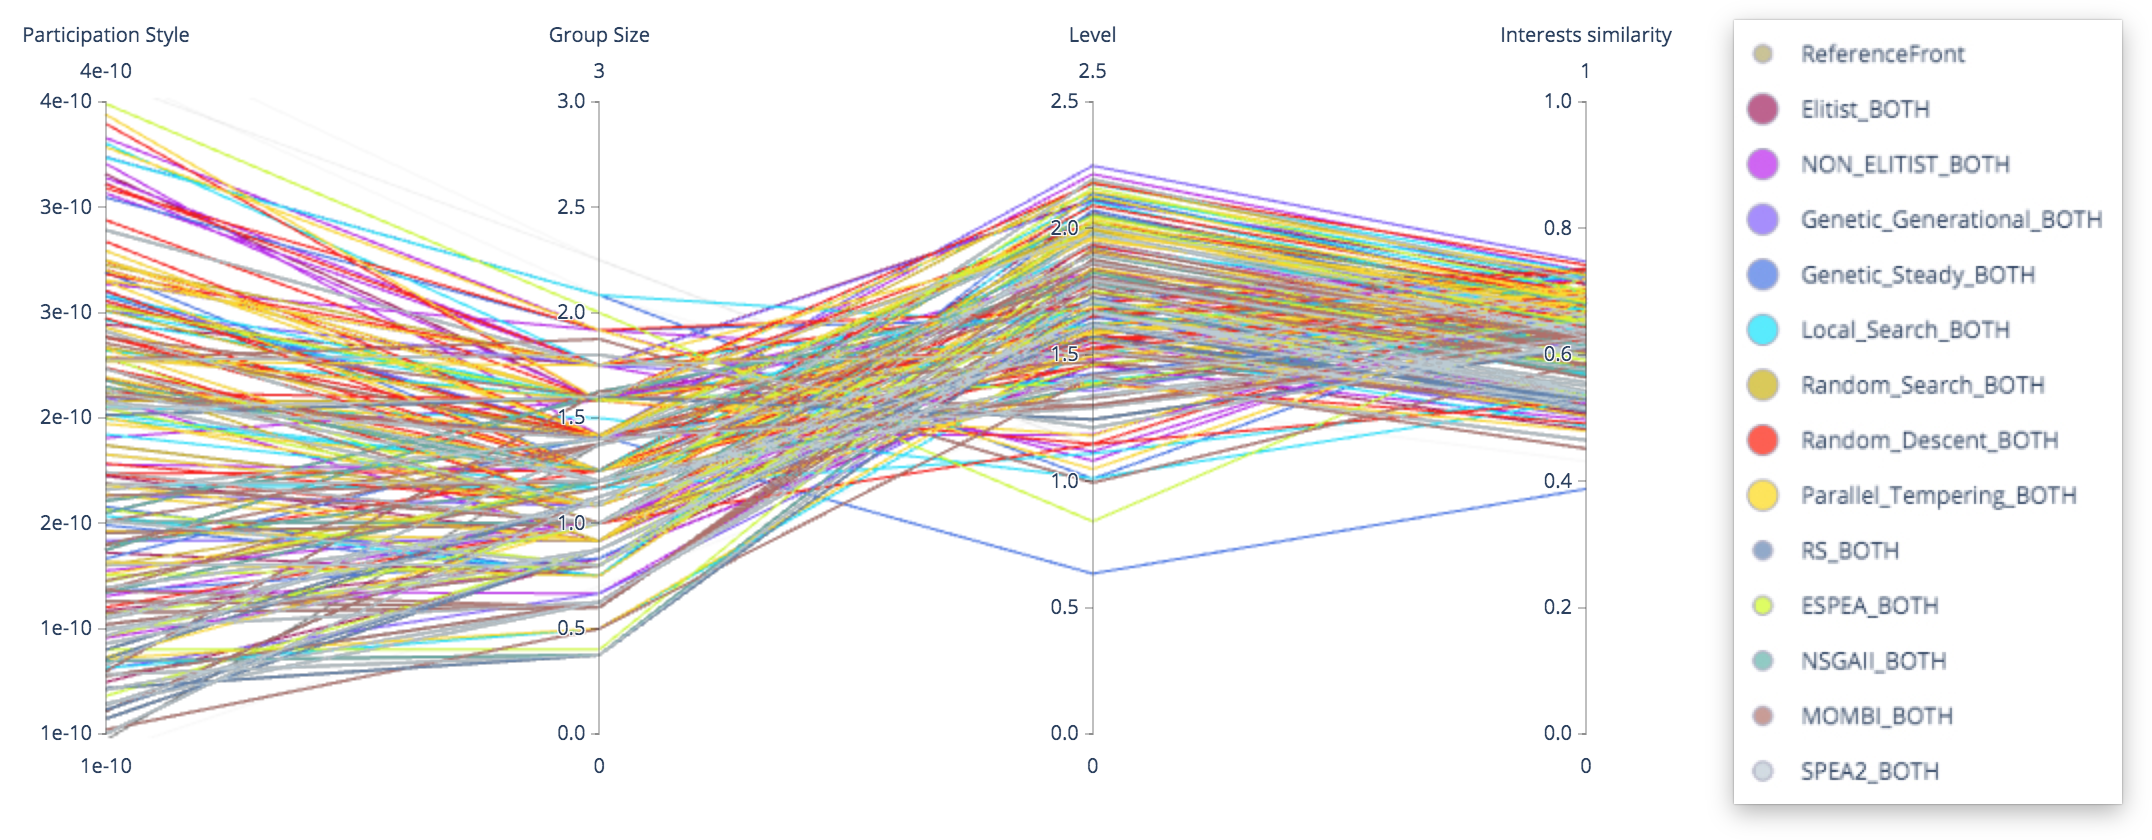
\includegraphics[width=\textwidth]{images/parallel_20.png}
    \caption{Results for the $n=20$ problem}
    \label{fig:parallel_20}
\end{figure}

Figure~\ref{fig:parallel_200} shows the results for the $n=200$. Here the SOA which are represented by the light colours are outperformed for the $Ps$ and $Gs$ objective functions, while SOA seems to outperform MOA for the $Lvl$ objective function and the $Int$ function is mostly dominated by MOA, although some SOAs were able to have similar or better results. The dominance of RS can also be more clearly seen in this Figure. Once again the reference front was overlapped by the results, it can be assumed that this was done by the MOA. There also seems to be a negative correlation between $Lvl$ and $Int$, this also seems the case for $Lvl$ and $Gs$.

\begin{figure}[H]
    \centering
    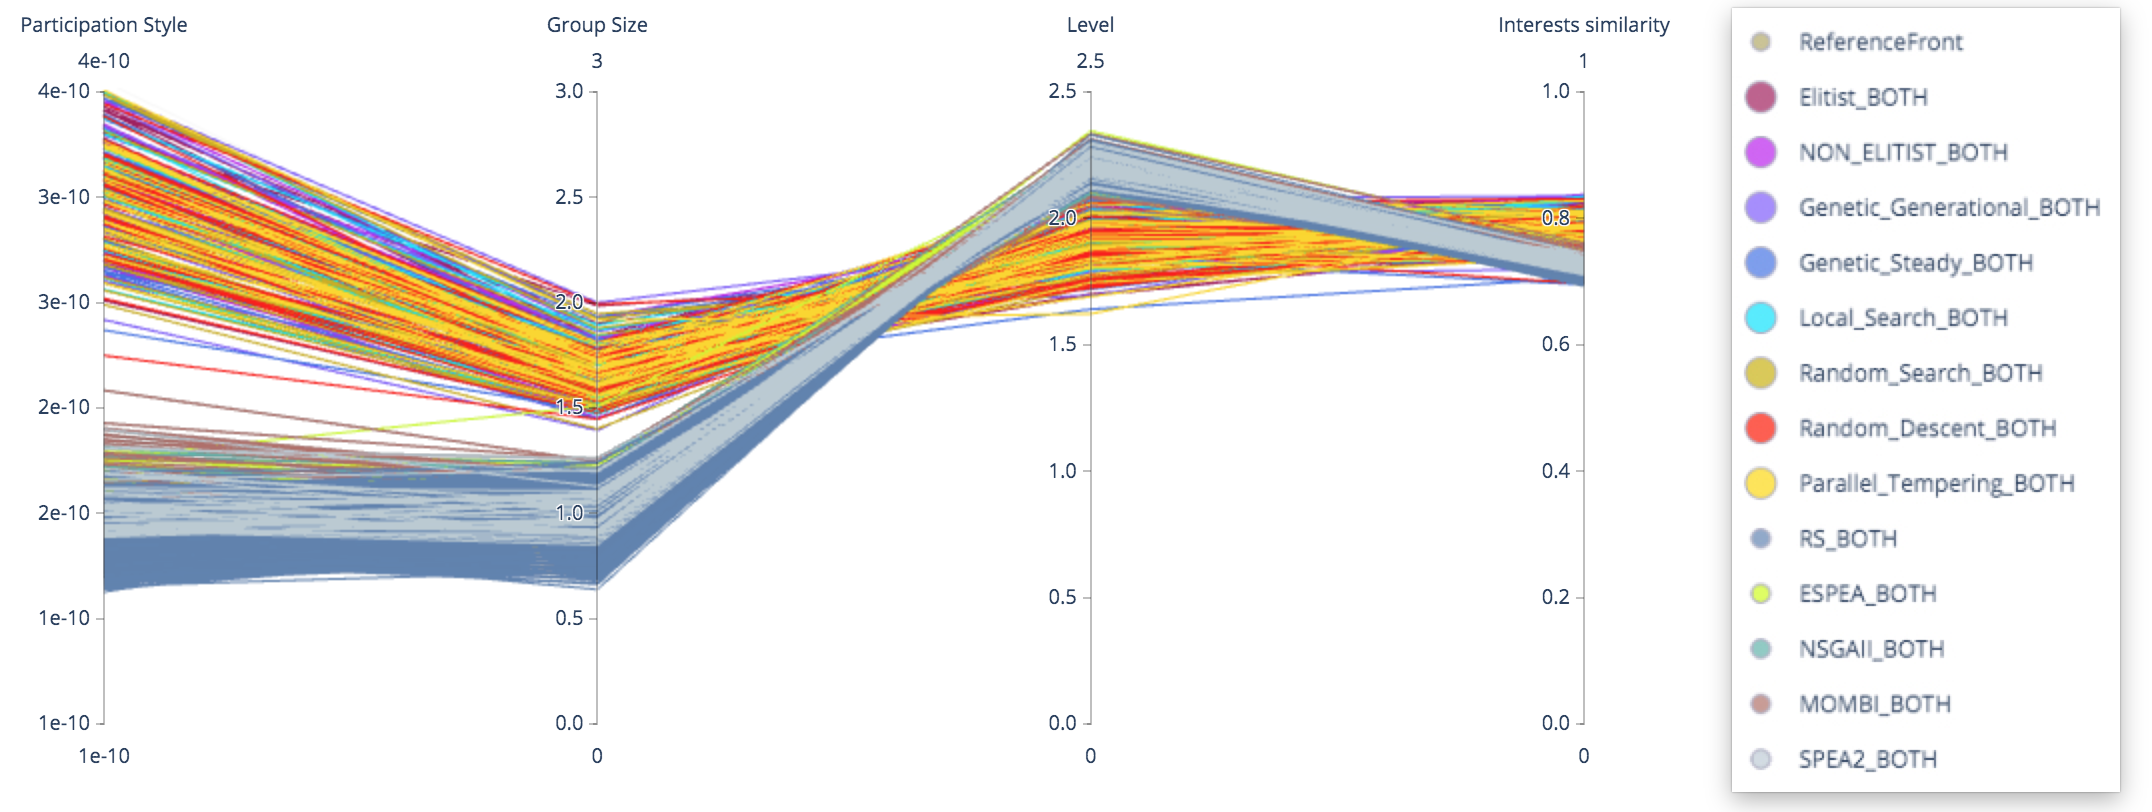
\includegraphics[width=\textwidth]{images/parallel_200.png}
    \caption{Results for the $n=200$ problem}
    \label{fig:parallel_200}
\end{figure}

For the $n=2,000$ problem seen in Figure~\ref{fig:parallel_2000} The separation between SOA and MOA is more evident. The behaviour is very similar to the $n=200$ problem, although the separation is significantly more for the $Ps$ and $Gs$ functions. There is also now a clear gap between SOA and MOA for the $Int$ function, Which means MOA were able to outperform SOA for all the objective functions except for $Lvl$. In this problem, the reference front can still be seen dominating the rest of the solutions, especially for the $Ps$ function.

\begin{figure}[H]
    \centering
    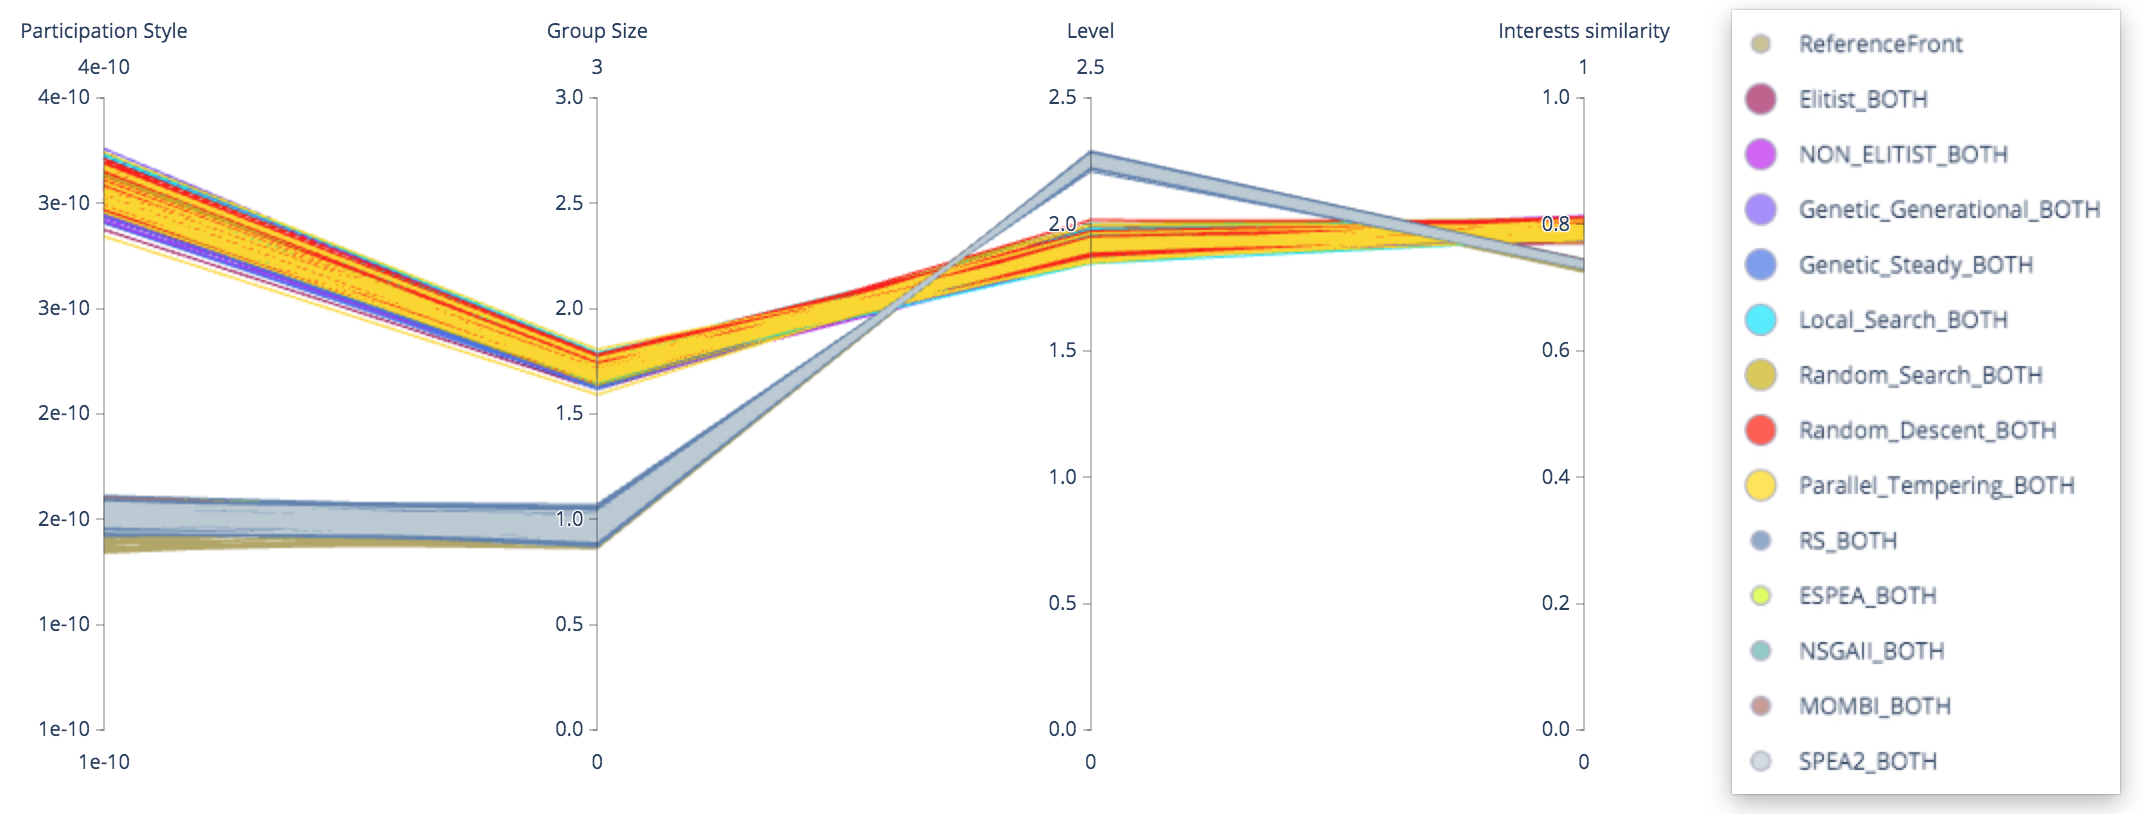
\includegraphics[width=\textwidth]{images/parallel_2000.png}
    \caption{Results for the $n=2,000$ problem}
    \label{fig:parallel_2000}
\end{figure}

By a visual comparison, there seems to be an advantage for RS outperforming most of the algorithms. One explanation for this can be that, as described in Section~\ref{sec:initialisation}, the initialisation has a random starting point and it varies for each independent run, the Mutation operator described in Section~\ref{section:mutation_operator} makes only small changes, and considering the search space the algorithms are not able to explore it conveniently. The search is restricted to a subspace that depends on the starting point, and therefore the problem is sensible to the starting solutions.

\subsection{Comparison between single-objective algorithms}

To determine the best SOA, a Friedman test was made. The results are shown in Table~\ref{table:fried_igdp_(MOA)}. The metric for comparison was $IGD+$, this is because of the previous discussion about the unreliability of $HV$ for the SOA. Here the algorithm which outperforms the rest seems to be PT with RS and NES as the ones to follow. One reason that can explain the performance of PT is the ability to search in parallel. Since the algorithm runs in parallel with different start solutions, and as previously mentioned, the problem seems to be very sensitive to the starting solutions, this allows PT to optimise different solutions and selecting the best solution in the end. The worst performing algorithm is RD this can be attributed the fact that the algorithm selects a random solution of its neighbourhood, despite being better or not, but since the change in each step is very small, the algorithm may get trapped in local minima frequently. However the Friedman test was made considering a $\alpha > 0.2$, so this comparison may not be significant.

% Single Objective Algorithms

% --------Friedman IGD+--------

\begin{table}[!htp]
    \centering
    \begin{threeparttable}
    \begin{tabular}{lc}
    \hline
    Algorithm&Ranking\\
    \hline
    Random Descent&5.75\\
    Parallel Tempering&3.00\\
    Random Search&3.75\\
    Local Search&4.50\\
    Genetic Steady&5.00\\
    Genetic Generational&5.25\\
    Elitist&5.00\\
    NON ELITIST&3.75\\
    \hline
    \end{tabular}
        \begin{tablenotes}
        \small
        \item Friedman statistic for the metric IGD+ considering reduction performance (distributed according to chi-square with 7 degrees of freedom: 4.00).
        \end{tablenotes}
    \end{threeparttable}
    \caption{Average ranking of the algorithms.}
    \label{table:fried_igdp_(SOA)}
\end{table}

\subsection{Comparison between multi-objective algorithms}

In a similar fashion to SOA, a Friedman test was also made for the MOA. Table~\ref{table:fried_igdp_(MOA)} shows RS as the best algorithm outperforming all the other MOA which could also be perceived visually by looking at the graphs in the previous subsection. Just as mentioned, this is likely because of the sensibility of the problem to the starting point, but this may also be an indication that there should be a fine-tuning for the parameters to outperform random sampling. MOMBI2 was considered the worst MOA, which could be attributed to it requiring more specific parameters. The test presented a $\alpha < 0.050$ which is considered as statistically significant.

% Multi-Objective Algorithms

\begin{table}[!htp]
    \centering
    \begin{threeparttable}
    \begin{tabular}{lc}
    \hline
    Algorithm~~~~~~&~~~~~Ranking\\
    \hline
    ESPEA&3.00\\
    MOMBI2&4.25\\
    NSGAII&3.00\\
    RS&1.00\\
    SPEA2&3.75\\
    \hline
    \end{tabular}
        \begin{tablenotes}
        \small
        \item Friedman statistic considering reduction performance (distributed according to chi-square with 4 degrees of freedom: 9.80).
        \end{tablenotes}
    \end{threeparttable}
    \caption{Average ranking of the algorithms.}
    \label{table:fried_igdp_(MOA)}
\end{table}

\subsection{Comparison between Single-Objective and Multi-Objective Algorithms}

The results of both SOA and MOA were combined to show which group of algorithms outperform the other. As previously stated, the SOA solutions seem to be separated from MOA solutions, although, for some of the solutions SOA is shown to outperform MOA. For the $n=200$ problem, the separation between MOA and SOA becomes clearer, and there is not any solution form SOA outperforming MOA, the $n=2,000$ problem, shows a similar behaviour, with the SOA solutions getting further away. There also seems to be a particular trade-off for the $Lvl$ and the $Ps$ functions, where SOA can obtain better performance for the $Lvl$ and MOA for the $Ps$ function.\\

To have a better understanding of the comparison between algorithms, an analysis was made using the mean and standard deviation of the $IGD+$ for all the algorithms. The results are shown in Table~\ref{tab:me_std_both_igdp}, having the mean of the results as the main number and the standard deviation as its suffix. The first thing to notice is that for the $n=20$ problem, RS has a metric of 0 which means it reached the reference front solution. For the $n=200$ and $n=2,000$ it came very close to it. The second best algorithm may vary according to the problem size, but for the $n=20$ problem, the results obtained by MOA are close to each other, however, for the $n=200$ there seems to be more variation. Then for the $n=2,000$ problem, the variation is low again, even getting closer to RS results. The performance of SOA seems to be consistent across each of the problems, interestingly just as MOA, there seems to be a better performance in reaching the reference front in the $n=2,000$ than $n=200$ problem.

\begin{table}[H]
    \centering
    {%\resizebox{\textwidth}{!}{%
    \begin{tabular}{lllll}
    \hline
    Algorithm & $n=20$ & $n=200$ & $n=2,000$ \\
    \hline
    ESPEA                & $  4.89_{ 4.00}$                   & \cellcolor{gray25}$  2.84_{ 2.60}$ & $  1.15_{ 0.57}$                  \\
    MOMBI2                & \cellcolor{gray25}$  3.59_{ 3.10}$ & $ 7.55_{ 5.20}$                    & $  1.85_{ 0.94}$                 \\
    NSGAII               & $  4.23_{3.50}$                   & $  4.23_{ 3.10}$                    & \cellcolor{gray25}$  1.12_{0.57}$ \\
    RS                   & \cellcolor{gray95}$ 0.00_{ 0.00}$ & \cellcolor{gray95}$  0.02_{0.02}$   & \cellcolor{gray95}$  0.76_{0.38}$ \\
    SPEA2                & $  4.94_{4.30}$                   & $   3.93_{3.40}$                    & $  1.31_{0.65}$                   \\
    Random Descent       & $  10.03_{4.80}$                  & $  30.58_{10.50}$                   & $  10.93_{7.20}$                  \\
    Parallel Tempering   & $  9.12_{5.10}$                   & $  30.62_{10.60}$                   & $  10.85_{7.50}$                  \\
    Random Search        & $  9.65_{4.20}$                   & $  30.52_{10.50}$                   & $  10.91_{7.10}$                  \\
    Local Search         & $  9.54_{4.80}$                   & $  30.69_{10.50}$                   & $  10.94_{7.30}$                  \\
    Genetic Steady       & $  9.91_{4.80}$                   & $  30.68_{10.50}$                   & $  10.90_{7.10}$                  \\
    Genetic Generational & $  9.84_{4.60}$                   & $  30.69_{10.50}$                   & $  10.90_{7.20}$                  \\
    Elitist              & $  9.83_{4.80}$                   & $  30.86_{10.60}$                   & $  10.91_{7.20}$                  \\
    NON ELITIST          & $  9.07_{5.60}$                   & $  30.58_{10.50}$                   & $  10.90_{7.20}$                  \\                
    \hline
    \end{tabular}%
    }
    \caption{Mean and Standard Deviation for the IGD+ metric.}
    \label{tab:me_std_both_igdp}
\end{table}
    
Another analysis using the median and interquartile range was made in the same fashion, the results are shown in Table~\ref{tab:me_int_both_igdp}. Here the results are very similar to the ones found in Table~\ref{tab:me_std_both_igdp}. However there is a noticeable change for the SOA in the $n=200$ and $n=2,000$ problems, this means there might be results that performed considerably better for the SOA, which seems to be the case, looking at the parallel plots from the previous section, where some SOA results performed even better than MOA, but this was not the overall case.

% Please add the following required packages to your document preamble:
% \usepackage{graphicx}
\begin{table}[H]
    \centering
    {%\resizebox{\textwidth}{!}{%
    \begin{tabular}{lllll}
    \hline
    Algorithm & $n=20$ & $n=200$ & $n=2,000$ \\
    \hline
    ESPEA                & $  4.96_{7.80}$                    & \cellcolor{gray25}$  2.29_{3.20}$    & $  1.42_{0.03}$                  \\
    MOMBI2                & \cellcolor{gray25}$  1.98_{6.10}$  & $  7.97_{ 9.50}$                     & $  2.13_{0.05}$                 \\
    NSGAII               & $  3.79_{7.00}$                    & $  3.86_{ 4.00}$                     & \cellcolor{gray25}$  1.34_{0.38}$\\
    RS                   & \cellcolor{gray95}$  0.00_{0.00}$  & \cellcolor{gray95}$  0.020_{ 0.04}$  & \cellcolor{gray95}$  0.92_{0.13}$\\
    SPEA2                & $  4.06_{7.40}$                   & $  2.82_{3.40}$                      & $  1.56_{0.34}$                  \\
    Random Descent       & $  10.19_{3.80}$                   & $  30.90_{ 10.10}$                   & $  20.20_{2.30}$                 \\
    Parallel Tempering   & $  10.10_{5.50}$                   & $  40.09_{ 10.00}$                   & $  20.14_{1.90}$                 \\
    Random Search        & $  10.10_{2.50}$                   & $  30.88_{ 10.00}$                   & $  20.16_{1.20}$                 \\
    Local Search         & $  10.09_{7.70}$                   & $  40.20_{ 10.00}$                   & $  20.21_{2.00}$                 \\
    Genetic Steady       & $  10.13_{5.20}$                   & $  40.31_{ 10.40}$                   & $  20.18_{1.90}$                 \\
    Genetic Generational & $  10.01_{3.80}$                   & $  40.01_{ 10.30}$                   & $  20.13_{2.30}$                 \\
    Elitist              & $  10.10_{4.30}$                   & $  40.33_{ 10.00}$                   & $  20.18_{2.00}$                 \\
    NON ELITIST          & $  10.09_{100.10}$                 & $  30.80_{ 10.30}$                   & $  20.17_{2.30}$                 \\                
    \hline
    \end{tabular}%
    }
    \caption{Median and interquartile Range for the IGD+.}
    \label{tab:me_int_both_igdp}
\end{table}

The final analysis between all the algorithms was made using a Friedman ranking, just as for the SOA and MOA alone. The results are shown in Table~\ref{tab:fried_both_igdp}. The ranking is mostly the same as it was done by the previous analysis. None of the SOA was able to outperform the MOA. This test presents a $\alpha < 0.0005$ which is considered statistically significant.

% --------Friedman IGD+--------

\begin{table}[H]
    \centering
    \begin{threeparttable}
    \begin{tabular}{lc}
    \hline
    Algorithm&Ranking\\
    \hline
    ESPEA&2.75\\
    MOMBI2&4.25\\
    NSGAII&3.00\\
    RS&1.00\\
    SPEA2&4.00\\
    Random Descent&10.00\\
    Parallel Tempering&8.75\\
    Random Search&8.5\\
    Local Search&9.75\\
    Genetic Steady&10.25\\
    Genetic Generational&10.75\\
    Elitist&9.75\\
    NON ELITIST&8.25\\
    \hline
    \end{tabular}
    \begin{tablenotes}
        \small
        \item Friedman statistic for the metric $IGD+$  considering reduction performance (distributed according to chi-square with 12 degrees of freedom: 37.51).\\
    \end{tablenotes}
    \end{threeparttable}
    \caption{Average ranking of the algorithms.}
    \label{tab:fried_both_igdp}
\end{table}

\subsection{Stability evaluation}

To test the stability, an experiment took place measuring the results from the previous set of exploratory experiments for the $n=20$ problem. The results were evaluated using the methodology described in Section~\ref{section:stability}. The number of stable users is considered for each preference criteria. And by each of the tested algorithms. The analysis was made using a metaheuristic LS, the single objective genetic algorithm GGA and the multi-objective algorithm NSGA-II. Using a random solution for comparison.\\

Results are shown in Table~\ref{tab:preference_criteria}, here the solutions obtained from the algorithms are compared to a random solution, it can be seen that the stability improves or stays the same for all the algorithms, except for the $Lvl$ criteria. This can be explained because of the little variation between the levels of the students. Interestingly, NSGA-II seems to have the most stability spread across all the objective functions.\\

% Please add the following required packages to your document preamble:
% \usepackage{graphicx}
\begin{table}[H]
\centering
\resizebox{\textwidth}{!}{%
\begin{tabular}{lcccc}
\hline
 & $Gs-Stable$ & $Ps-Stable$ & $Int-Stable$ & $Lvl-Stable$ \\
 \hline
Random Solution & 3 & 0 & 0 & 12 \\
Local Search & 6 & 3 & 0 & 7 \\
Genetic Generational Algorithm & 8 & 0 & 2 & 7 \\
NSGA-II & 3 & 2 & 2 & 9 \\
\hline
\end{tabular}%
}
\caption{Number of stable students in the groups by preference criteria}
\label{tab:preference_criteria}
\end{table}

This analysis was made not to test which algorithm lead to the most stability, but to ensure that by optimising the objective functions it can lead to higher stability. However, in future research, it might be possible to have a deeper analysis of the behaviour of the stability of this problem.
    
\section{Second Phase}

After receiving some feedback about phase one, there was the discussion if the SOA and MOA were comparing the same objectives. To prove this another set of experiments was proposed. First, an experiment took place which consisted in building a Pareto front using each function individually with every SOA, to check if the SOA would have an advantage optimising each objective separately. Then, an evaluation using a Chebyshev scalarization function took place.\\

\subsection{Pareto Front Construction from Single Objective Algorithms}
\label{sec:front_construction}

For this experiment, each SOA evaluated each one of the objective functions independently across {30} independent runs. The results were then combined to build a Front that resembling a Pareto Front.\\ 

Visual results for the $n=20$ problem can be seen in Figure~\ref{fig:front_mixed_20} once again are unclear, since all the solutions overlap each other. This presents a similar behaviour to the one found in the first phase in Section~\ref{sec:first_phase}. The spread of the solutions cover more space in this case because each different algorithm is optimising something different.\\

\begin{figure}[H]
    \centering
    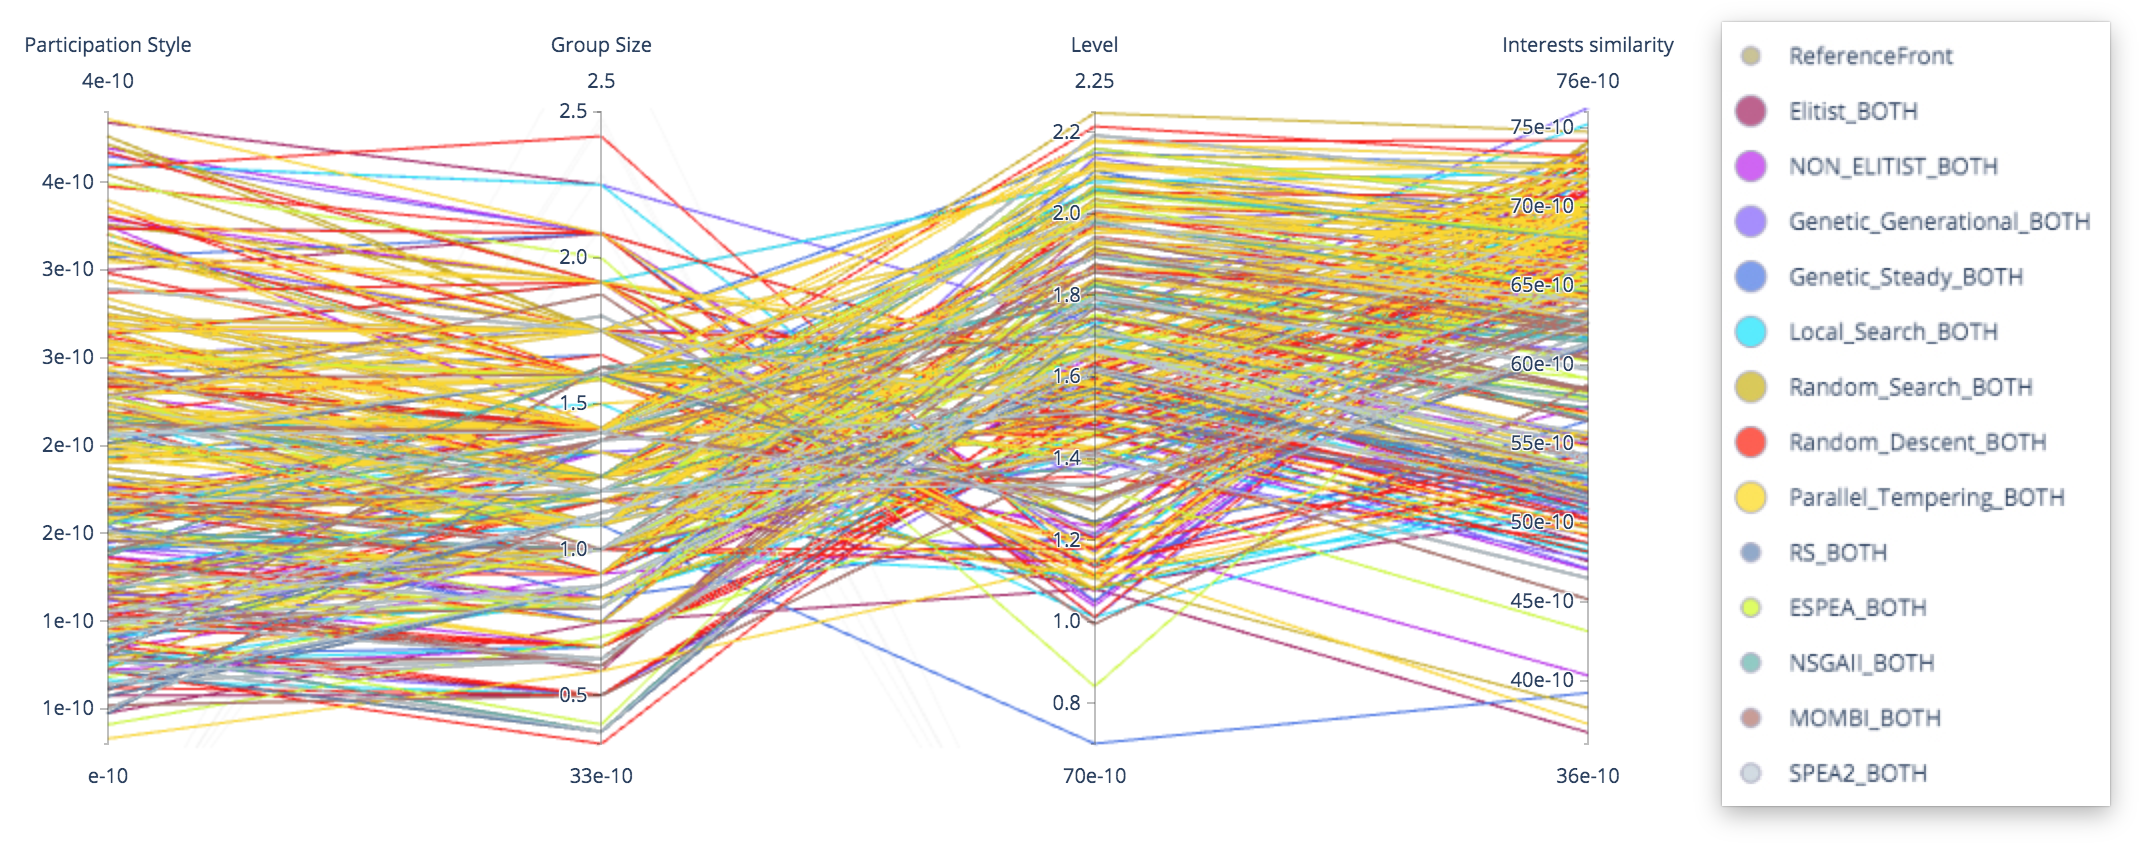
\includegraphics[width=\textwidth]{images/mixed_front_20.png}
    \caption{Results for the $n=20$ problem, optimising each objective function individually}
    \label{fig:front_mixed_20}
\end{figure}

For the problem $n=200$, the results are shown in Figure~\ref{fig:front_mixed_200}. Here the results seem to be very similar to the ones found in the previous experiment. This behaviour was suspicious because there is known that there are better results for each of the objective functions, but for some reason SOA was not able to reach these results. The experiment was run again, meticulously checking each configuration, showing similar results. This shows further evidence of a characteristic of MOA that make them able to outperform SOA.

\begin{figure}[H]
    \centering
    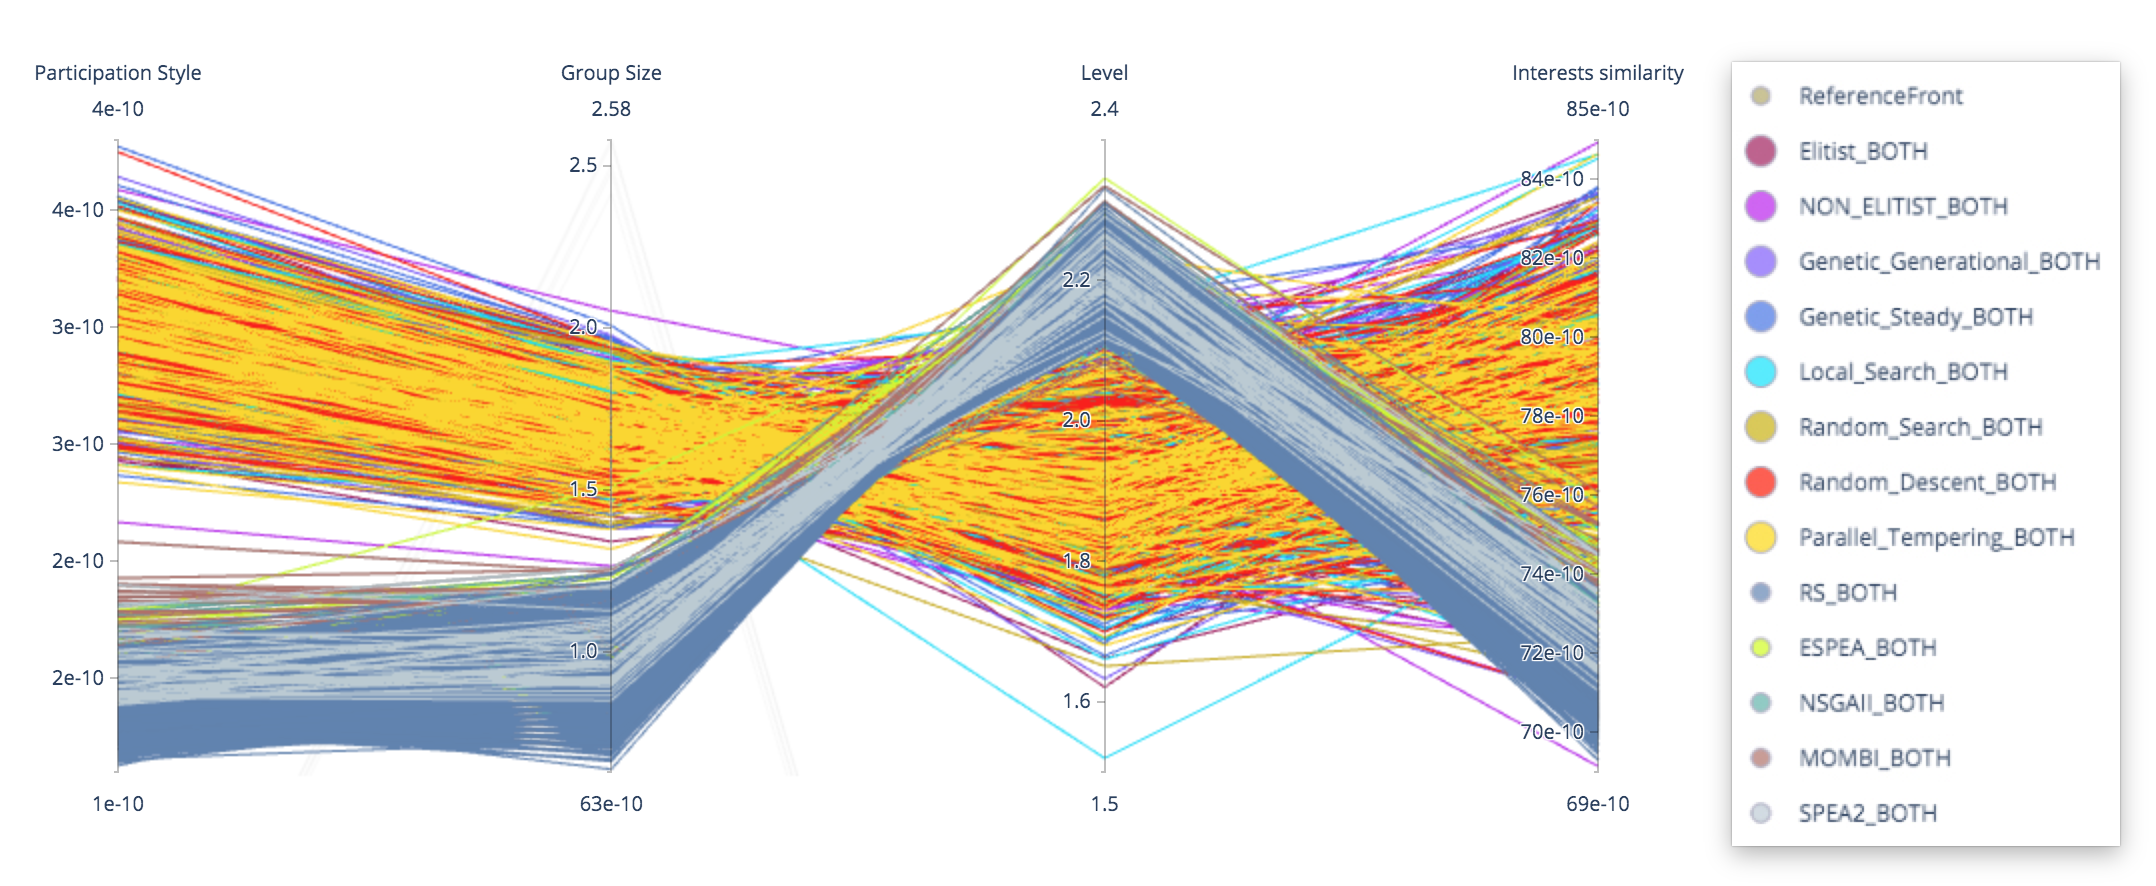
\includegraphics[width=\textwidth]{images/mixed_front_200.png}
    \caption{Results for the $n=200$ problem, optimising each objective function individually}
    \label{fig:front_mixed_200}
\end{figure}

Results for the $n=2,000$ problem shown in Figure~\ref{fig:front_mixed_2000}, also present a similar behaviour to the previous experiment, despite of the different objectives. This experiment was also run one more time checking the configuration, just as for the $n=200$ problem, and it also had similar results.

\begin{figure}[H]
    \centering
    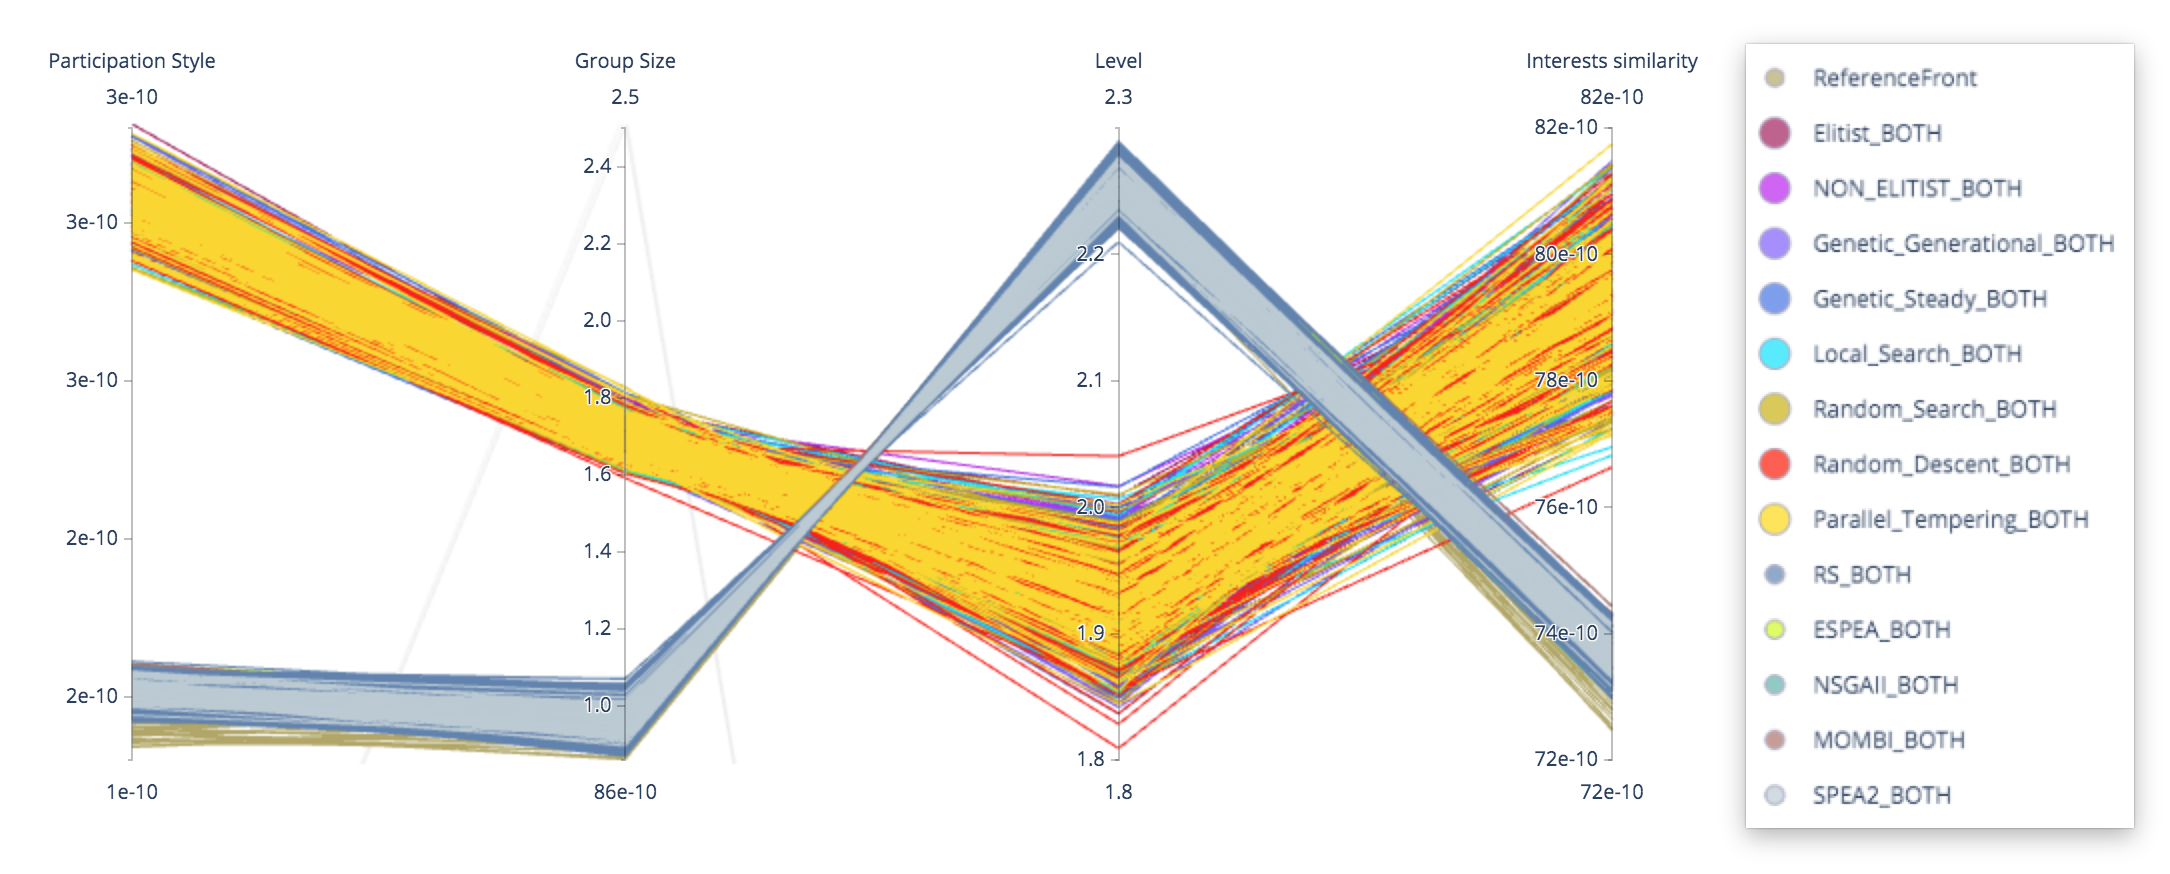
\includegraphics[width=\textwidth]{images/mixed_front_2000.png}
    \caption{Results for the $n=2,000$ problem, optimising each objective function individually}
    \label{fig:front_mixed_2000}
\end{figure}

The analysis of the mean and standard deviation, seen in Figure~\ref{tab:me_std_mix_igdp} shows an improvement of the SOA for the $n=20$ problem, even being able to successfully outperform all MOA, except for RS. The second best algorithm is now ES and all SOA get very close to the reference front. However, this advantage is lost with the $n=200$ problem. Although it still has a better performance compared to the previous experiment. Results for the $n=2,000$ remain mostly the same. This analysis was made by building a single front with the SOA and comparing it with the previous results, so it did not make sense to include the standard deviation, median and interquartile range as with the previous analysis.

% --------IGD+--------

% Please add the following required packages to your document preamble:
% \usepackage{graphicx}
\begin{table}[H]
    \centering
    {%\resizebox{\textwidth}{!}{%
    \begin{tabular}{lllll}
    \hline
    Algorithm & $n=20$ & $n=200$ & $n=2,000$ \\
    \hline
    ESPEA                & $  4.89$                    & \cellcolor{gray25}$  2.84$ & $  1.15$                  \\
    MOMBI2               & $  3.59$                    & $ 7.55$  & $  1.85$                 \\
    NSGAII               & $  4.23$                    & $  4.23$                    & \cellcolor{gray25}$  1.12$   \\
    RS                   & \cellcolor{gray95}$ 0.00$   & \cellcolor{gray95}$  0.02$   & \cellcolor{gray95}$  0.76$  \\
    SPEA2                & $  4.94$                    & $   3.93$                    & $   1.31$                   \\
    Random Descent       & $  0.05$                    & $  20.82$                    & $  10.86$                   \\
    Parallel Tempering   & $  0.06$                    & $  20.47$                    & $  10.84$                   \\
    Random Search        & $  0.70$                    & $  20.73$                    & $  10.86$                   \\
    Local Search         & $  0.13$                    & $  20.66$                    & $  10.83$                   \\
    Genetic Steady       & $  0.39$                    & $  20.54$                    & $  10.86$                   \\
    Genetic Generational & $  0.13$                    & $  20.81$                    & $  10.93$                   \\
    Elitist              & \cellcolor{gray25}$  0.04$ & $  20.69$                    & $  10.93$                   \\
    NON ELITIST          & $  0.29$                    & $  20.04$                    & $  10.87$                   \\
    \hline
    \end{tabular}%
    }
    \caption{IGD+. Mean and Standard Deviation.}
    \label{tab:me_std_mix_igdp}
\end{table}

As with the previous experiment, a Friedman ranking took place which results are shown in Table~\ref{tab:fried_mix_igd}. Compared to the previous results there is a clear improvement for the SOA, coming very close for the ranking, especially in the case of LS. However, once again, none of the SOA was able to outperform MOA. The test presents a $\alpha < 0.0005$ which is considered statistically significant.

% --------Friedman IGD+--------

\begin{table}[H]
    \centering
    \begin{threeparttable}
    \begin{tabular}{lc}
    \hline
    Algorithm&Ranking\\
    \hline
    ESPEA&5.50\\
    MOMBI2&6.00\\
    NSGAII&5.50\\
    RS&1.00\\
    SPEA2&4.75\\
    Random Descent&9.50\\
    Parallel Tempering&7.25\\
    Random Search&9.75\\
    Local Search&6.75\\
    Genetic Steady&9.5\\
    Genetic Generational&9.75\\
    Elitist&8.25\\
    NON ELITIST&7.5\\
    \hline
    \end{tabular}
    \begin{tablenotes}
        \small
        \item Friedman statistic for the metric $IGD+$ considering reduction performance (distributed according to chi-square with 12 degrees of freedom: 20.07).\\
        \end{tablenotes}
    \end{threeparttable}
    \caption{Average ranking of the algorithms for the metric IGD+.}
    \label{tab:fried_mix_igd}
\end{table}

\subsection{Chebyshev Scalarization Function}

Another criticism about SOA and MOA comparison about the scalarization function, since it was established earlier in this section that both SOA and MOA were optimising different things. Using each objective function as individual functions for optimisation in the last experiment brought a more fair comparison, however, it performed poorly since the fronts generated did not consider the rest of the objective problems for optimisation. To address this issue, a Chebyshev scalarization function was used as the objective function in a new set of experiments.\\

To use the Chebyshev Scalarization function it was necessary to use a combination of weights that allowed the exploration of the search space similar to the multi-objective approach. With a different weight for each objective function that changes for each different run, recreating a Pareto front. The weights considered where $0.1$, $0.2$, $0.3$ and $0.4$ their summation results in $1.0$. Since there are 4 different weights all the permutations of them were considered corresponding to a different run for each. In total there were $24$ independent runs for the $n=20$, $n=200$ and $n=2,000$ problems.\\

A visualisation of the results can be seen in Figure~\ref{fig:front_chebyshev_20}. Differently from the previous results, there is a clear advantage of SOA against MOA for the $Lvl$ function. Results for the $Ps$ and $Gs$ objective functions seem to be mostly the same, however SOA now presents a slight advantage for the $Gs$ function. The $Int$ function dominance fairly shared among SOA and MOA, although now SOA seems to have had an improvement over the previous experiment.

\begin{figure}[H]
    \centering
    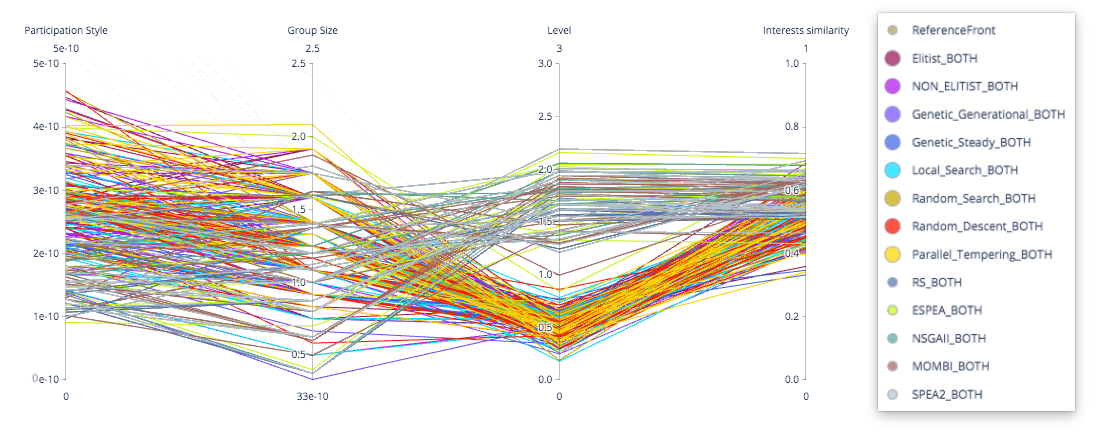
\includegraphics[width=\textwidth]{images/chebyshev_20.png}
    \caption{Results for the $n=20$ problem, optimising the Chebyshev scalarization function}
    \label{fig:front_chebyshev_20}
\end{figure}

The results for the $n=200$ problem shown in Figure~\ref{fig:front_chebyshev_200} show a clearer distinction between SOA and MOA. Solutions for SOA considering the $Ps$ and $Gs$ functions remain mostly the same. The most noticeable difference is with $Lvl$ function, the previous experiment showed a slight advantage for the SOA, but it now has improved even further. The $Int$ function is now dominated by SOA, but some MOA still have competent results.

\begin{figure}[H]
    \centering
    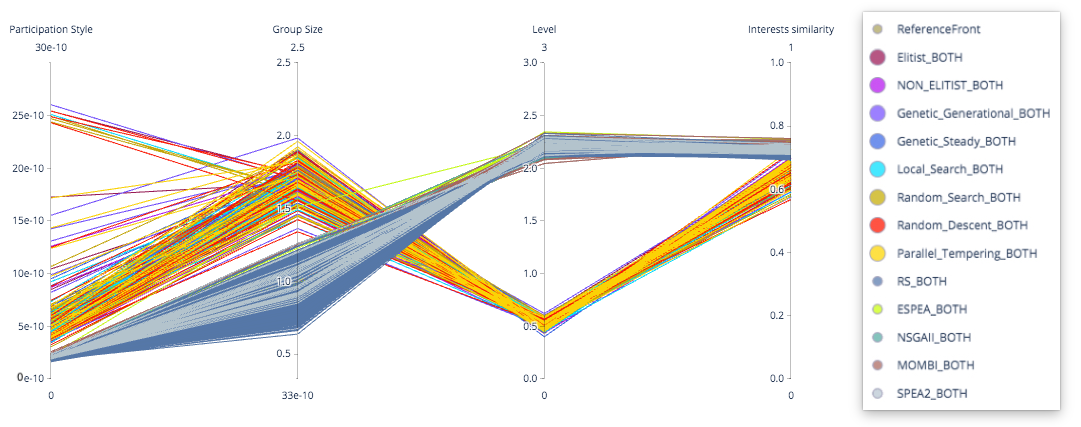
\includegraphics[width=\textwidth]{images/chebyshev_200.png}
    \caption{Results for the $n=200$ problem, optimising the Chebyshev scalarization function}
    \label{fig:front_chebyshev_200}
\end{figure}

The visualisation of the $n=2,000$ problem, shown in Figure~\ref{fig:front_chebyshev_2000}. Here, once again is the same for the $Gs$ function, $Ps$ seems to have decreased in comparison to the previous experiment. The results for the $Lvl$ are concentrated in a value. Also, The gap between SOA and MOA considering the $Int$ function is now much more noticeable.

\begin{figure}[H]
    \centering
    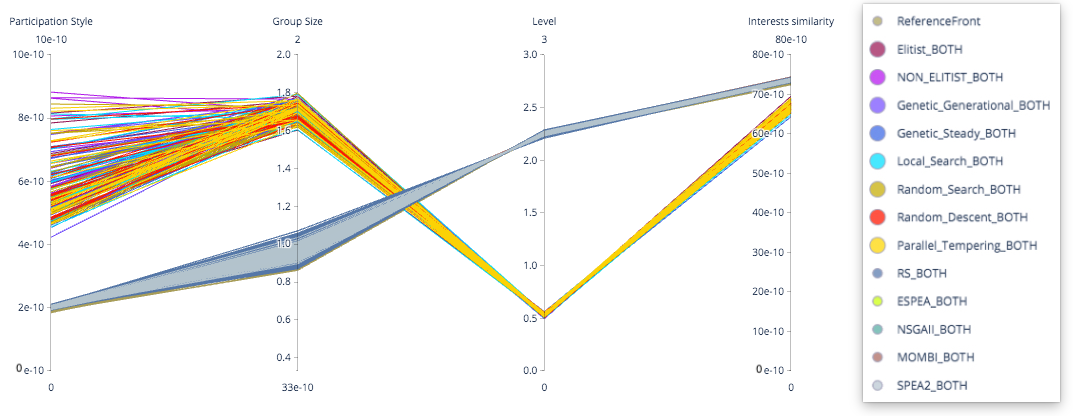
\includegraphics[width=\textwidth]{images/chebyshev_2000.png}
    \caption{Results for the $n=2000$ problem, optimising the Chebyshev scalarization function}
    \label{fig:front_chebyshev_2000}
\end{figure}

An analysis of the mean and the standard deviation can be seen in Table~\ref{tab:me_std_che_igdp}. There is a slight improvement over the previous experiment in the $n=20$ problem for the SOA, although still none of them was able to outperform MOA. For the $n=200$ problem, the Mean of $IGD+$ metric is very high compared to MOA. This was also observed in Figure\ref{fig:front_chebyshev_200}, where some of the results of SOA performed poorly in the $Ps$ function. For the $n=2,000$ the results are also worse, however not as bad as for the $n=200$ problem.

\begin{table}[H]
    \centering
    {%\resizebox{\textwidth}{!}{%
    \begin{tabular}{lllll}
    \hline
    Algorithm & $n=20$ & $n=200$ & $n=2,000$ \\
    \hline
    ESPEA                & $  4.89_{ 4.00}$                   & \cellcolor{gray25}$  2.84_{ 2.60}$ & $  1.15_{ 0.57}$                  \\
    MOMBI2                & \cellcolor{gray25}$  3.59_{ 3.10}$ & $ 7.55_{ 5.20}$                    & $  1.85_{ 0.94}$                 \\
    NSGAII               & $  4.23_{3.50}$                   & $  4.23_{ 3.10}$                    & \cellcolor{gray25}$  1.12_{0.57}$ \\
    RS                   & \cellcolor{gray95}$ 0.00_{ 0.00}$ & \cellcolor{gray95}$  0.02_{0.02}$   & \cellcolor{gray95}$  0.76_{0.38}$ \\
    SPEA2                & $  4.94_{4.30}$                   & $   3.93_{3.40}$                 & $  1.31_{0.65}$                      \\
    Random Descent       & $7.49_{ 4.20}$                      & $  142.00_{ 170.00}$            & $  46.80_{ 10.00}$              \\
    Parallel Tempering   & $7.25_{ 2.50}$                      & $  114.00_{  87.00}$            & $  45.70_{ 13.00}$              \\
    Random Search        & $7.37_{ 3.70}$                      & $  144.00_{ 170.00}$            & $  44.10_{ 11.00}$              \\
    Local Search         & $5.98_{ 4.10}$                      & $  108.00_{ 100.00}$            & $  47.30_{ 12.00}$              \\
    Genetic Steady       & $7.34_{ 5.60}$                      & $   84.80_{  39.00}$            & $  42.40_{  9.00}$              \\
    Genetic Generational & $7.18_{ 4.70}$                      & $  129.00_{ 130.00}$            & $  44.60_{  9.60}$              \\
    Elitist              & $7.33_{ 2.70}$                      & $  116.00_{ 120.00}$            & $  47.00_{ 10.00}$              \\
    NON ELITIST          & $6.90_{ 4.60}$                      & $   78.10_{  49.00}$            & $  50.00_{ 14.00}$              \\
    \hline
    \end{tabular}%
    }
    \caption{IGD+. Mean and Standard Deviation.}
    \label{tab:me_std_che_igdp}
\end{table}

The analysis of median and interquartile range, shown in Table~\ref{tab:me_int_che_igdp} shows that the median is lower for some SOA solutions for the $n=20$ problem, this means the mean previously obtained was affected by low performing solutions. This seems to be also the case for the $n=200$ problem although the solutions obtained are still worse than the ones found in the previous experiment. The $n=2,000$ problem seems to be very consistent with the mean analysis presented above.

% Please add the following required packages to your document preamble:
% \usepackage{graphicx}
\begin{table}[H]
    \centering
    {%\resizebox{\textwidth}{!}{%
    \begin{tabular}{lllll}
    \hline
    Algorithm & $n=20$ & $n=200$ & $n=2,000$ \\
    \hline
    ESPEA                & $  4.96_{7.80}$                    & \cellcolor{gray25}$  2.29_{3.20}$    & $  1.42_{0.03}$                  \\
    MOMBI2               & \cellcolor{gray25}$  1.98_{6.10}$  & $  7.97_{ 9.50}$                     & $  2.13_{0.05}$                 \\
    NSGAII               & $  3.79_{7.00}$                    & $  3.86_{ 4.00}$                     & \cellcolor{gray25}$  1.34_{0.38}$\\
    RS                   & \cellcolor{gray95}$  0.00_{0.00}$  & \cellcolor{gray95}$  0.020_{ 0.04}$  & \cellcolor{gray95}$  0.92_{0.13}$\\
    SPEA2                & $  4.06_{7.40}$                   & $  2.82_{3.40}$                      & $  1.56_{0.34}$                  \\
    Random Descent       & $  6.22_{ 4.10}$ & $  67.30_{ 78.00}$ & $42.60_{ 19.00}$  \\
    Parallel Tempering   & $  7.02_{ 4.50}$ & $  80.40_{ 66.00}$ & $39.60_{ 17.00}$  \\
    Random Search        & $  6.07_{ 4.70}$ & $  90.90_{ 63.00}$ & $40.90_{ 16.00}$  \\
    Local Search         & $  5.40_{ 2.80}$ & $  86.30_{ 39.00}$ & $44.40_{ 15.00}$  \\
    Genetic Steady       & $  5.33_{ 2.80}$ & $  74.90_{ 55.00}$ & $39.50_{ 16.00}$  \\
    Genetic Generational & $  5.71_{ 7.00}$ & $  78.10_{ 93.00}$ & $41.00_{ 15.00}$  \\
    Elitist              & $  6.68_{ 4.40}$ & $  66.50_{ 49.00}$ & $42.40_{ 16.00}$  \\
    NON ELITIST          & $  5.78_{ 4.90}$ & $  61.50_{ 32.00}$ & $45.40_{ 18.00}$  \\
    \hline
    \end{tabular}%
    }
    \caption{IGD+. Median and Interquartile Range.}
    \label{tab:me_int_che_igdp}
\end{table}

A Friedman Ranking test was made, comparing the results of these experiments with the previous results. This is shown in Table~\ref{tab:fried_che_igd}. In this test, SOA perform similarly to the previous experiment, some Algorithms like LS, GSA and GGA perform better. Overall none of the SOA was able to outperform MOA. This was done with a $\alpha < 0.0005$ which is considered statistically significant. 

% --------Friedman IGD+--------

\begin{table}[H]
    \centering
    \begin{threeparttable}
    \begin{tabular}{lc}
    \hline
    Algorithm&Ranking\\
    \hline
    ESPEA&3.00\\
    MOMBI2&4.00\\
    NSGAII&2.66\\
    RS&1.00\\
    SPEA2&4.66\\
    Random Descent&11.66\\
    Parallel Tempering&9.00\\
    Random Search&10.66\\
    Local Search&8.33\\
    Genetic Steady&8.00\\
    Genetic Generational&9.00\\
    Elitist&10.33\\
    NON ELITIST&8.66\\
    \hline
    \end{tabular}
    \begin{tablenotes}
        \small
        \item Friedman statistic for the metric $IGD+$ considering reduction performance (distributed according to chi-square with 12 degrees of freedom: 28.70).\\
        \end{tablenotes}
    \end{threeparttable}
    \caption{Average ranking of the algorithms for the metric IGD+.}
    \label{tab:fried_che_igd}
\end{table}

While the overall analysis indicates that MOA outperforms SOA even considering the recommended improvements, shows a clear indication that MOA has some characteristics that allow them to converge, cover better the search space, hence they can escape local minima. However, the Analysis using Chebyshev scalarization function showed that there is a possibility to tune the parameters and have consistently better results. This opens the possibility to explore it further in the future.

\section{Third Phase}

As already established in phase one and phase two, MOA outperformed SOA starting from a {200} size problem, and mostly outperformed them also in the smaller problem of {20}. However, according to the Friedman test, the algorithm that outperformed all the algorithms overall was RS which meant that no optimisation was taken place, just random solutions outperforming each other.\\

This suggests that there is an opportunity for additional parameter tuning. Therefore for this last set of experiments, it was considered only the two other best algorithms from MOA which were ESPEA and NSGA-II. These were adjusted according to a set of parameters according to the ones used to obtain the best performance for SMP found in~\cite{bello2016genetic}, which consisted in a more aggressive mutation of {0.8} and a lower setting for the crossover rate of {0.5}. Also, it was applied a rule of thumb indicating to use {7} to {10} times the size of the problem for the population to have better coverage for the search space~\cite{kazimipour2014effects}. Finally, other variations for these algorithms were also tested, using different replacement strategies for ESPEA and different variations of the NSGA-II algorithm. Like the last phase, these experiments were only tested for the {20} and {200} data-set sizes.\\

The visual representation of the results are shown in Figure~\ref{fig:3d_smp_20} for the $n=20$ problem. ESPEA showed a noticeable poor performance compared to NSGA-II and RS. The algorithm NSGA-II and its variations seem to have a performance comparable to RS, however, RS seems to overlap NSGA-II results, so the conclusions may need to be better checked with the numerical evaluations since visually it cannot draw any conclusions. Both RS and NSGA-II seem to have gone further from the reference front.

\begin{figure}[H]
    \centering
    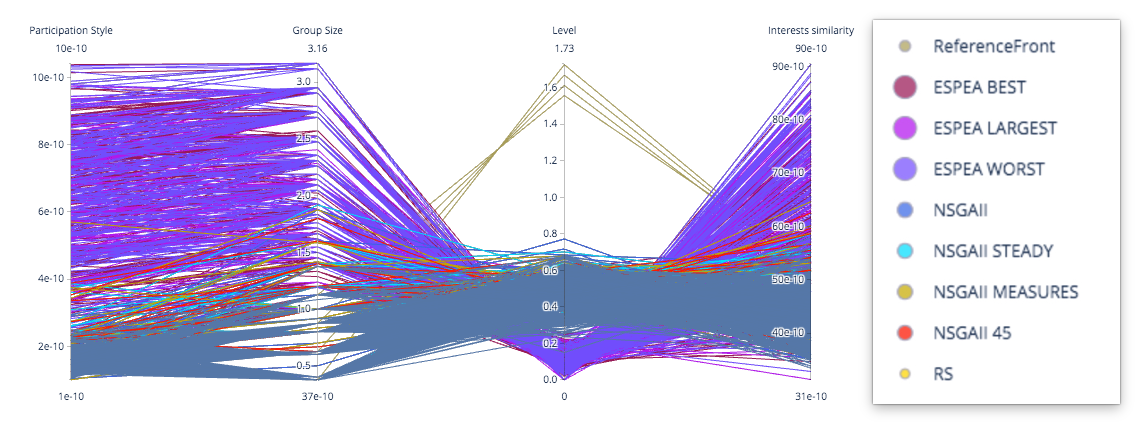
\includegraphics[width=\textwidth]{images/smp_20.png}
    \caption{Visualisation of the $n=20$ problem, using SMP parameters}
    \label{fig:3d_smp_20}
\end{figure}

For the $n=200$ problem, seen in Figure\ref{fig:3d_smp_200}, there is a more evident gap between ESPEA and NSGA-II and RS. Some of the results the variation of NSGA-II, NSGAII 45, has results that perform slightly worse than RS for the $Gs$ function. Once again the established reference front has been surpassed by RS and NSGA-II algorithms.

\begin{figure}[H]
    \centering
    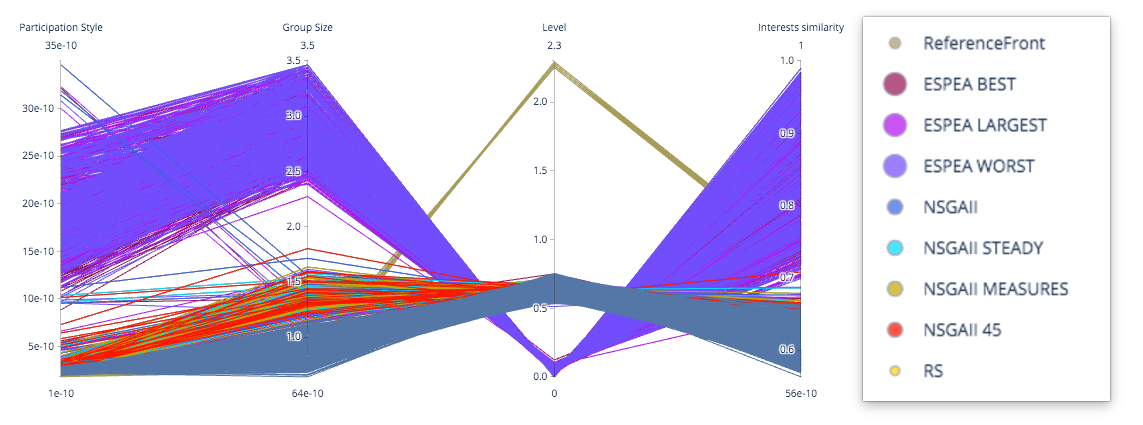
\includegraphics[width=\textwidth]{images/smp_200.png}
    \caption{Visualisation of the $n=200$ problem, using SMP parameters}
    \label{fig:3d_smp_200}
\end{figure}

Since this last comparison is made with only MOA algorithms, and since some of the algorithms have surpassed the reference front, it the $HV$ which is the most frequent metric for MOA comparison is used instead of $IGD+$. The Mean and Standard Deviation analysis is shown in Table~\ref{tab:me_std_smp_hv} shows an advantage for the NSGA-II and its variations against ESPEA and RS. The previous visualisation has all the results of RS shown in a single colour. However, it is important to remember that these results may belong to different fronts, which indicates that the results are inconsistent for RS. This realisation makes sense, since RS has a random nature, and in comparison NSGA-II can produce more competitive results.

% --------HV--------

% Please add the following required packages to your document preamble:
% \usepackage{graphicx}
\begin{table}[H]
    \centering
    {%\resizebox{\textwidth}{!}{%
    \begin{tabular}{lll}
    \hline
    Algorithm & $n = 20$ & $n = 200 $ \\
    \hline
    ESPEA BEST & $  1.13e+03_{ 2.9e+02}$ & $  3.47e+05_{ 6.6e+05}$ \\
    ESPEA LARGEST & $  1.07e+03_{ 5.4e+02}$ & $  3.25e+05_{ 2.4e+05}$ \\
    ESPEA WORST & $  1.16e+03_{ 4.8e+02}$ & $  4.63e+05_{ 1.1e+06}$ \\
    NSGAII & \cellcolor{gray95} $6.50e+01_{ 6.7e+01}$ & $  1.65e+05_{ 3.2e+05}$ \\
    NSGAII STEADY & \cellcolor{gray25} $  6.92e+01_{ 9.3e+01}$ & $  6.04e+04_{ 8.9e+04}$ \\
    NSGAII MEASURES & $9.65e+01_{ 1.6e+02}$ & \cellcolor{gray95} $4.07e+04_{ 2.1e+04}$ \\
    NSGAII 45 & $  8.27e+01_{ 9.1e+01}$ & \cellcolor{gray25} $  5.30e+04_{ 4.8e+04}$ \\
    RS & $  2.31e+02_{ 2.3e+02}$ & $  3.30e+05_{ 9.7e+04}$ \\
    \hline
    \end{tabular}%
    }
    \caption{HV. Mean and Standard Deviation.}
    \label{tab:me_std_smp_hv}
\end{table}
    
The median and interquartile range analysis is shown in Table~\ref{tab:me_int_smp_hv} is consistent with the mean and standard deviation analysis. It can also be noticed that for some algorithms the median is considerably lower than the mean, which means that some of the results might have been considerably worse, lowering their performance for the mean analysis. Despite this the most competitive results still belong to the NSGA-II variations, considering specifically the "Measures" variation the algorithm with consistently better results for this analysis.
    
% Please add the following required packages to your document preamble:
% \usepackage{graphicx}
\begin{table}[H]
    \centering
    {%\resizebox{\textwidth}{!}{%
    \begin{tabular}{lll}
    \hline
    Algorithm & $n = 20$ & $n = 200 $ \\
    \hline
    ESPEA BEST & $  1.09e+03_{ 4.3e+02}$ & $  2.34e+05_{ 1.7e+05}$ \\
    ESPEA LARGEST & $  1.10e+03_{ 5.8e+02}$ & $  2.53e+05_{ 1.7e+05}$ \\
    ESPEA WORST & $  1.05e+03_{ 7.0e+02}$ & $  2.86e+05_{ 1.1e+05}$ \\
    NSGAII & $  5.44e+01_{ 8.2e+01}$ & $  4.33e+04_{ 5.2e+04}$ \\
    NSGAII STEADY & \cellcolor{gray25} $  4.29e+01_{ 9.2e+01}$ & $  3.85e+04_{ 2.7e+04}$ \\
    NSGAII MEASURES & \cellcolor{gray95} $  2.86e+01_{ 1.0e+02}$ & \cellcolor{gray95} $  3.47e+04_{ 3.3e+04}$ \\
    NSGAII 45 & $  4.72e+01_{ 1.1e+02}$ & \cellcolor{gray25} $  3.55e+04_{ 3.7e+04}$ \\
    RS & $  1.66e+02_{ 2.8e+02}$ & $  3.32e+05_{ 1.1e+05}$ \\
    \hline
    \end{tabular}%
    }
    \caption{HV. Median and interquartile range.}
    \label{tab:me_int_smp_hv}
\end{table}

A Friedman ranking test took place, just as with the previous experiments, with its results shown in Table~\ref{tab:fried_smp_hv}. Here all the NSGA-II variations have the same ranking that overall show a better performance, successfully surpassing RS. Interestingly the ESPEA variation with the "Largest" replacement strategy comes very close in the ranking to RS. This ranking considers a $\alpha > 0.0.075$, so this comparison is considered as statistically significant.

% --------Friedman HV--------

\begin{table}[H]
    \centering
    \begin{threeparttable}
    \begin{tabular}{lc}
    \hline
    Algorithm&Ranking\\
    \hline
    ESPEA BEST&7.00\\
    ESPEA LARGEST&5.50\\
    ESPEA WORST&8.00\\
    NSGAII&2.50\\
    NSGAII STEADY&2.50\\
    NSGAII MEASURES&2.50\\
    NSGAII 45&2.50\\
    RS&5.05\\
    \hline
    \end{tabular}
    \begin{tablenotes}
        \small
        \item Friedman statistic for the metric $HV$ considering reduction performance (distributed according to chi-square with 7 degrees of freedom: 12.16).
        \end{tablenotes}
    \end{threeparttable}
    \caption{Average ranking of the algorithms for the metric HV.}
    \label{tab:fried_smp_hv}
\end{table}
    
% - NSGAII was finally able to outperform RS using X parameters with an improvement in its Hypervolume.

\section{Correlation between the results}

After extensive analysis and looking at the results and observing an apparent trade-off between some of the objective functions There was the need of analysing the correlation among objectives over the non-dominated, which were taken from the best front obtained from the $n=200$ problem.\\

For this correlation analysis, a Pearson's Correlation test was used taking into account all the objective functions results and their correlation between each other.

% Please add the following required packages to your document preamble:
% \usepackage{graphicx}
\begin{table}[H]
\centering

\begin{tabular}{lll}
\hline
Objective Functions & Statistic & P-value \\
\hline
Group Size and Participation Style & $0.50$ & $2.17e-08$ \\
Group Size and Level & $-0.96$ & $2.04e-17$ \\
Group Size and Interests Similarity & $-0.57$ & $4.57e-11$ \\
Participation Style and Level & $-0.55$ & $3.26e-10$ \\
Participation Style and Interests Similarity & $0.03$ & $0.74$ \\
Level and Interests Similarity & $0.69$ & $2.04e-17$ \\
\hline
\end{tabular}%

\caption{Results of the Pearson correlation analysis}
\label{tab:correlation}
\end{table}

Taking the results from Table~\ref{tab:correlation}, The null Hypothesis of being two independent sets is rejected in all the comparisons except for the $Ps$ and the $Int$ functions using a less than one per cent significance. This means All the objective functions are correlated except for these two. However, for the $Gs$ in respect to the $Lvl$ and $Int$, there seems to be a negative correlation, the same with the $Ps$ and $Lvl$. This was also observed visually in Figure~\ref{fig:parallel_2000} and others, where SOA seem to achieve better results for the $Lvl$ and MOA better results for the $Ps$ function.\\

It also makes sense for the $Gs$  to be correlated to the $Ps$ since the more members are in a group since the more people are in the group, the more participation will take place in the group. $Gs$ and $Lvl$ are negatively correlated, which also makes sense, since the higher the members of the group.
This also validates more the use of MOA over SOA, since there are at least two objective functions which are not correlated.